% for 16x9 (modern wide screen) aspect ratio slides
\documentclass[aspectratio=169]{beamer}

% Oxford Maths theming
\usetheme{oxfordmaths}
\usepackage{xcolor}

% ===== Semantic color palette =====
% Observed data (empirical / from experiment)
\colorlet{colData}{green!20}
\colorlet{colDataLine}{green!50!black}
% ODE / differentiable modules
\colorlet{colODE}{blue!12}
\colorlet{colODELine}{blue!70!black}
% Stochastic / simulation modules
\colorlet{colSim}{orange!12}
\colorlet{colSimLine}{orange!70!black}
% Posteriors / inference output
\colorlet{colPost}{violet!15}
\colorlet{colPostLine}{violet!70!black}
% Infrastructure / neutral
\colorlet{colNeutral}{gray!15}
% Problems / no-UQ / fragile
\colorlet{colWarn}{red!15}
\colorlet{colWarnLine}{red!70!black}

\hypersetup{colorlinks=true, urlcolor=teal, linkcolor=., filecolor=.}
\titlelogo{posterior_plot/posterior_plot.pdf}

% Set author etc info
\title[InferCell]{InferCell: Inference-First Whole-Cell Modelling}
\author{Tom Kimpson}
\institute{University of Melbourne}
\date[2026]{MACSYS Research Theme 1 Workshop, May 2026}

% ===== Packages & helpers =====
\usepackage{amsmath, amssymb, mathtools}
\usepackage{booktabs}
\usepackage{siunitx}
\usepackage{tikz}
\usepackage{pgfplots}
\pgfplotsset{compat=1.18}
\usetikzlibrary{arrows.meta, positioning, calc, decorations.pathreplacing, shapes.geometric, fit}
\usepackage{graphicx}
\graphicspath{{../}}
\usepackage{colortbl}
\usepackage{listings}

% Pre-define TikZ styles
\tikzset{
	modbox/.style={draw, rounded corners=4pt, minimum height=0.9cm, minimum width=2.2cm, font=\small, thick},
	inferbox/.style={draw, rounded corners=4pt, minimum height=0.7cm, font=\footnotesize, dashed, thick},
	pipelinebox/.style={draw, rounded corners, minimum height=0.8cm, font=\small, fill=#1},
	pipelinearr/.style={->, thick, >=stealth},
	brace/.style={decorate, decoration={brace, amplitude=6pt}},
}

% Julia code listing style
\lstdefinestyle{julia}{
	language=Python, % close enough for keywords
	basicstyle=\ttfamily\scriptsize,
	keywordstyle=\color{blue!70!black}\bfseries,
	stringstyle=\color{green!50!black},
	commentstyle=\color{gray},
	showstringspaces=false,
	columns=fullflexible,
	morekeywords={struct, function, end, using, abstract, type},
}

% Reduce cluttered bullets
\setbeamertemplate{itemize items}[circle]
\setbeamertemplate{enumerate items}[default]

% Backup slide commands to exclude appendix from total count
\newcommand{\backupbegin}{
	\newcounter{framenumberappendix}
	\setcounter{framenumberappendix}{\value{framenumber}}
}
\newcommand{\backupend}{
	\setcounter{framenumber}{\value{framenumberappendix}}
}

% Page number template
\makeatletter
\setbeamertemplate{page number in head/foot}{%
	\insertframenumber
}
\makeatother


\begin{document}

% ===== Title =====
\begin{frame}[plain]
	\titlepage
\end{frame}




% ================================================================
% SECTION 1: The Problem
% ================================================================
\section{The Problem}



% ----------------------------------------------------------------
\begin{frame}{Whole-Cell Models: The State of the Art}
	\begin{columns}[T]
		\begin{column}{0.55\textwidth}
			\begin{itemize}\itemsep6pt
				\item Representative SOTA WCM: Luthey-Schulten Lab's 4D model (MC4D, \textit{Cell} 2026)
				\begin{itemize}\itemsep3pt
					\item 493 genes, 4 coupled solvers
					\item 3D spatial resolution at 10\,nm voxels
					\item GPU-accelerated, full cell cycle
				\end{itemize}

%\item {\color{gray}\scriptsize Lattice Microbes (C++), LSODA (C/Python), LAMMPS (CUDA) --- coupled via Python glue}
			\end{itemize}
		\end{column}
		\begin{column}{0.42\textwidth}
			\centering
			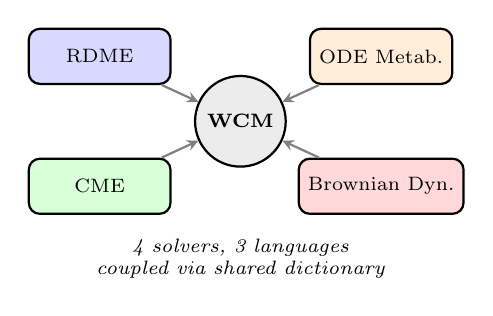
\begin{tikzpicture}[scale=0.55, every node/.style={font=\scriptsize}]
				% Four solver boxes around the outside
				\node[draw, rounded corners=4pt, thick, fill=blue!15, minimum height=0.7cm, minimum width=1.8cm, font=\scriptsize] (rdme) at (-1.5,3.5) {RDME};
				\node[draw, rounded corners=4pt, thick, fill=orange!15, minimum height=0.7cm, minimum width=1.8cm, font=\scriptsize] (ode) at (5,3.5) {ODE Metab.};
				\node[draw, rounded corners=4pt, thick, fill=green!15, minimum height=0.7cm, minimum width=1.8cm, font=\scriptsize] (cme) at (-1.5,0.5) {CME};
				\node[draw, rounded corners=4pt, thick, fill=red!15, minimum height=0.7cm, minimum width=1.8cm, font=\scriptsize] (bd) at (5,0.5) {Brownian Dyn.};
				% Central coordinator
				\node[draw, circle, thick, fill=gray!15, minimum size=1cm, font=\scriptsize] (sim) at (1.75,2) {\textbf{WCM}};
				% Arrows
				\draw[pipelinearr, gray] (rdme) -- (sim);
				\draw[pipelinearr, gray] (ode) -- (sim);
				\draw[pipelinearr, gray] (cme) -- (sim);
				\draw[pipelinearr, gray] (bd) -- (sim);
				% Label
				\node[below, font=\scriptsize\itshape, text width=4.5cm, align=center] at (1.75,-0.5) {4 solvers, 3 languages\\coupled via shared dictionary};
			\end{tikzpicture}
		\end{column}
	\end{columns}
\end{frame}

% SPEAKER NOTES:
% - MC4D runs 50 replicate simulations (15,000 GPU-hours on A100s), which captures
%   stochastic variation but NOT parameter uncertainty -- every replicate uses the
%   same fixed parameter values.
% - Direct quote from Thornburg et al. (2026): "no one organism has a complete set
%   of experimentally determined kinetic parameters ... the model has depended on
%   the transferability of quantities among related organisms"
% - Promoter strengths are parameterised from quantitative proteomics (direct
%   mapping, not formal inference). Some rates recalculated from M. pneumoniae.
% - No Bayesian inference, no posteriors, no formal UQ anywhere in the paper.




% ----------------------------------------------------------------
\begin{frame}{WCMs are Forward Simulators}
	\begin{columns}[T]
		\begin{column}{0.42\textwidth}
			\centering
			\vspace*{0.6cm}
			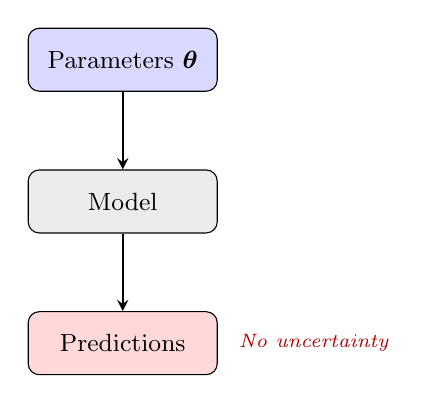
\begin{tikzpicture}[scale=0.9]
				\node[pipelinebox=blue!15, minimum width=2.4cm] (p) at (0,0) {Parameters $\boldsymbol{\theta}$};
				\node[pipelinebox=gray!15, minimum width=2.4cm] (m) at (0,-2.0) {Model};
				\node[pipelinebox=red!15, minimum width=2.4cm] (d) at (0,-4.0) {Predictions};
				\draw[pipelinearr] (p) -- (m);
				\draw[pipelinearr] (m) -- (d);
				% No UQ
				\node[font=\scriptsize\itshape, text=red!70!black, anchor=west] at (1.5,-4.0) {No uncertainty};
			\end{tikzpicture}
		\end{column}
			\begin{column}{0.55\textwidth}
			\centering
			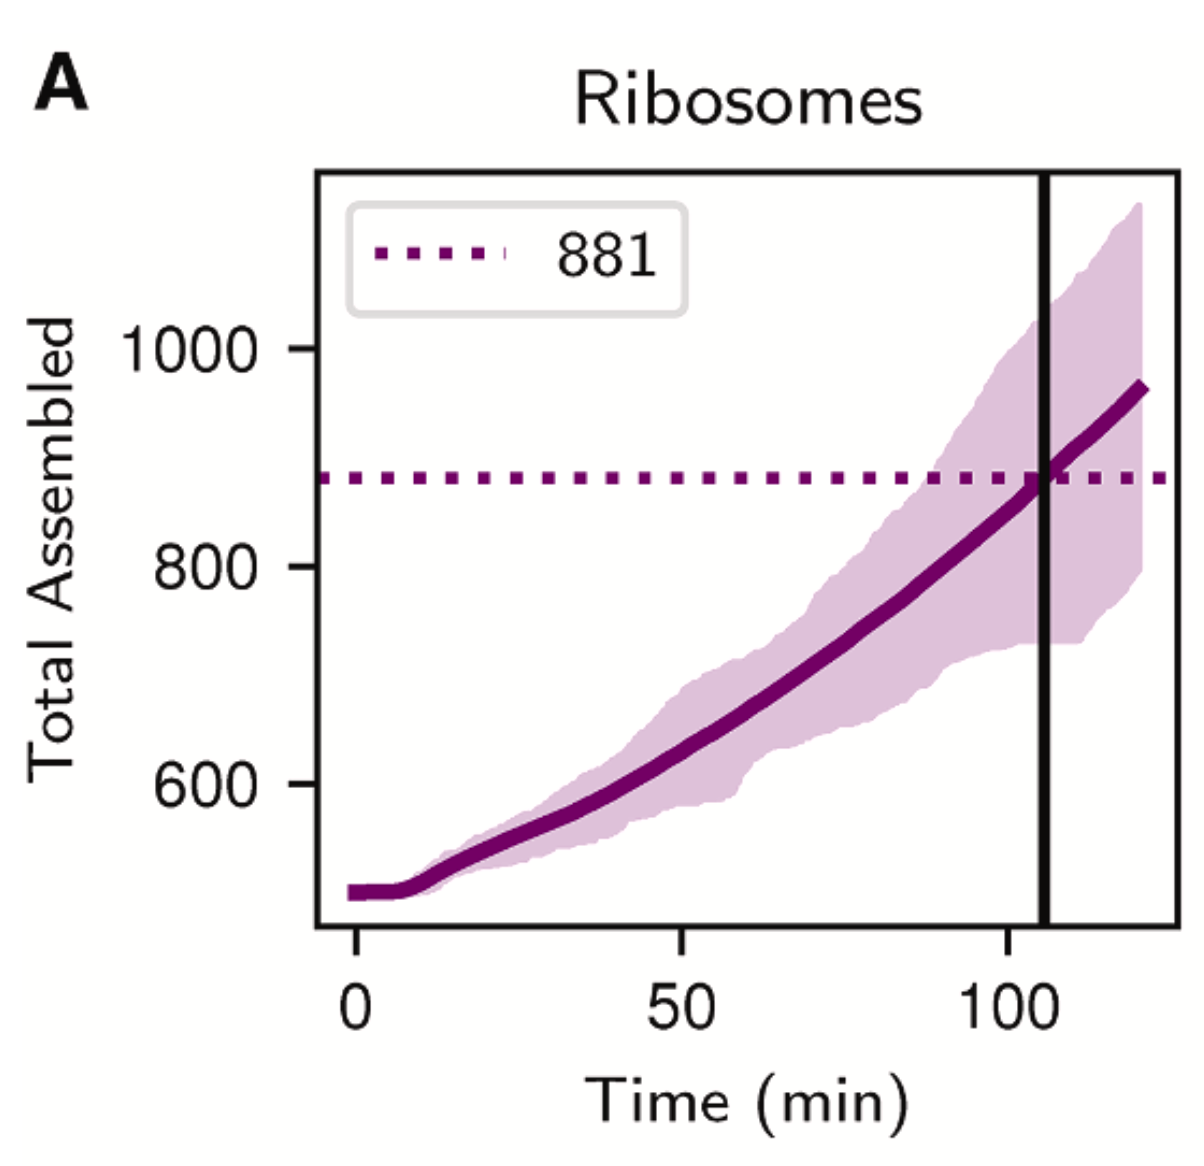
\includegraphics[width=0.75\columnwidth]{figures/ribosomes_plot.png}\\[4pt]
			{\scriptsize\itshape From \href{https://www.cell.com/cell/fulltext/S0092-8674(26)00174-1}{Thornburg et al., \textit{Cell} 2026}, Fig.~5}
		\end{column}
	\end{columns}

\end{frame}


% ----------------------------------------------------------------
\begin{frame}{But the parameters themselves are uncertain (epistemic uncertainty)}
	\begin{columns}[T]
		\begin{column}{0.55\textwidth}
			\begin{enumerate}\itemsep8pt
				\item \textbf{Parameters are uncertain.}\\
				{\small Rate constants from different organisms, conditions, experiments. Typical uncertainty: 10--50\%+.}
				\item \textbf{Uncertainty propagates nonlinearly.}\\
				{\small Uncertain rates $\to$ mRNA $\to$ protein $\to$ flux $\to$ growth rate.}
				\item \textbf{The architecture has no place to put it.}\\
				{\small MC4D stores parameters as names $\to$ floats. No distributions, no uncertainty.}
			\end{enumerate}
		\end{column}
		\begin{column}{0.42\textwidth}
			\centering
			% What we pretend - point estimate on a number line
			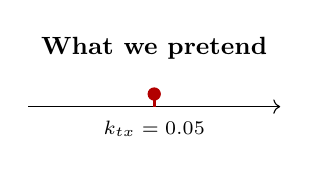
\begin{tikzpicture}[scale=0.8]
				\node[font=\small\bfseries, anchor=south] at (2,1.0) {What we pretend};
				\draw[->] (0,0.4) -- (4,0.4);
				\draw[very thick, red!70!black] (2,0.4) -- (2,0.6);
				\fill[red!70!black] (2,0.6) circle (3pt);
				\node[font=\scriptsize] at (2,0.05) {$k_{tx} = 0.05$};
			\end{tikzpicture}

			\vspace{8pt}

			% What we actually know - square histogram
			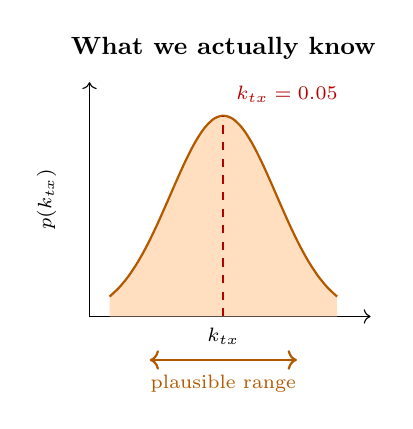
\begin{tikzpicture}[scale=0.85]
				\node[font=\small\bfseries, anchor=south] at (2,3.7) {What we actually know};
				\draw[->] (0,0) -- (4.2,0);
				\draw[->] (0,0) -- (0,3.5);
				\node[font=\scriptsize, rotate=90, anchor=south] at (-0.35,1.75) {$p(k_{tx})$};
				\fill[orange!25] plot[smooth, domain=0.3:3.7] (\x, {3.0*exp(-0.8*(\x-2)^2)}) -- (3.7,0) -- (0.3,0) -- cycle;
				\draw[thick, orange!70!black] plot[smooth, domain=0.3:3.7] (\x, {3.0*exp(-0.8*(\x-2)^2)});
				% Dashed vertical line at the point estimate
				\draw[dashed, thick, red!70!black] (2,0) -- (2,3.0);
				\node[font=\scriptsize, red!70!black, anchor=south west] at (2.05,3.05) {$k_{tx} = 0.05$};
				\node[font=\scriptsize] at (2,-0.3) {$k_{tx}$};
				\draw[<->, thick, orange!70!black] (0.9,-0.65) -- (3.1,-0.65);
				\node[font=\scriptsize, orange!70!black] at (2,-1.0) {plausible range};
			\end{tikzpicture}
		\end{column}
	\end{columns}
\end{frame}
% VERBAL: When MC4D predicts a 110-minute doubling time, we cannot distinguish
% whether (a) the prediction is robust across plausible parameters, or
% (b) it is fragile and depends on specific choices.






% ----------------------------------------------------------------
\begin{frame}{What Does That Uncertainty Look Like?}
	A minimal model with two parameters:
	$\;\dfrac{d[\text{mRNA}]}{dt} = k_{tx} - \gamma \cdot [\text{mRNA}]
	\;\;\Rightarrow\;\;
	[\text{mRNA}]_{ss} = k_{tx}/\gamma$

	\medskip
	\centering
	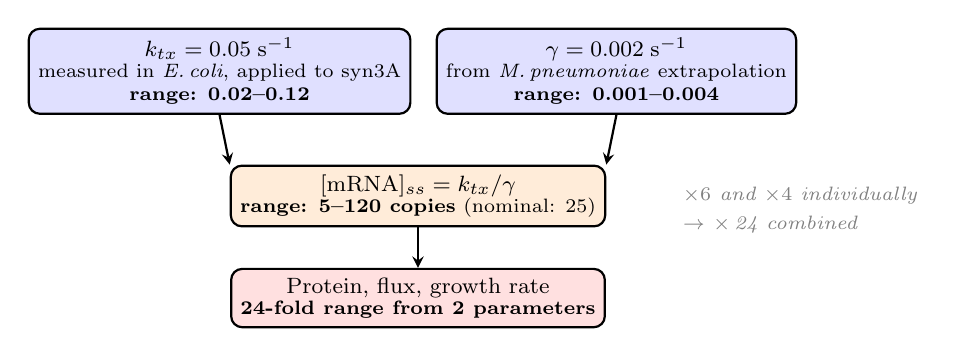
\begin{tikzpicture}[
		scale=0.72,
		box/.style={draw, thick, rounded corners=4pt, minimum height=0.7cm, align=center, font=\footnotesize},
		>=Stealth
	]
		% Parameter uncertainties
		\node[box, fill=blue!12, minimum width=3.4cm] (ktx) at (0,0) {$k_{tx} = 0.05 \;\text{s}^{-1}$\\[-2pt]\scriptsize measured in \textit{E.\,coli}, applied to syn3A\\[-1pt]\scriptsize \textbf{range: 0.02--0.12}};
		\node[box, fill=blue!12, minimum width=3.4cm] (gam) at (7,0) {$\gamma = 0.002 \;\text{s}^{-1}$\\[-2pt]\scriptsize from \textit{M.\,pneumoniae} extrapolation\\[-1pt]\scriptsize \textbf{range: 0.001--0.004}};

		% mRNA steady state
		\node[box, fill=orange!15, minimum width=4cm] (mrna) at (3.5,-2.2) {$[\text{mRNA}]_{ss} = k_{tx}/\gamma$\\[-2pt]\scriptsize \textbf{range: 5--120 copies} (nominal: 25)};

		% Downstream
		\node[box, fill=red!12, minimum width=4cm] (prot) at (3.5,-4) {Protein, flux, growth rate\\[-2pt]\scriptsize \textbf{24-fold range from 2 parameters}};

		% Arrows
		\draw[pipelinearr] (ktx.south) -- (mrna.north west);
		\draw[pipelinearr] (gam.south) -- (mrna.north east);
		\draw[pipelinearr] (mrna) -- (prot);

		% Annotations
		\node[font=\scriptsize\itshape, text=gray, anchor=west] at (8,-2.2) {$\times 6$ and $\times 4$ individually};
		\node[font=\scriptsize\itshape, text=gray, anchor=west] at (8,-2.7) {$\to$ $\times$\,24 combined};
	\end{tikzpicture}

%	\vfill
%	\raggedright Two parameters. One equation. Twenty-four-fold uncertainty in predictions.\\
%	MC4D has \textbf{${\sim}$2000 parameters} feeding coupled nonlinear dynamics.
\end{frame}

% ----------------------------------------------------------------
\begin{frame}{No information flows between modules}
	\centering
	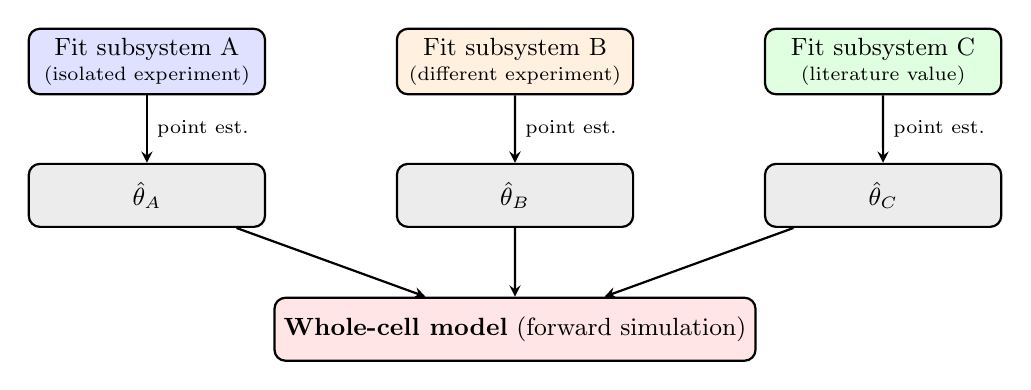
\begin{tikzpicture}[
		scale=0.85,
		wfbox/.style={draw, thick, rounded corners=4pt, minimum height=0.8cm, minimum width=3cm, align=center, font=\small},
		>=Stealth
	]
		% Isolated fits
		\node[wfbox, fill=blue!12] (fitA) at (0,2) {Fit subsystem A\\[-2pt]\scriptsize (isolated experiment)};
		\node[wfbox, fill=orange!12] (fitB) at (5.5,2) {Fit subsystem B\\[-2pt]\scriptsize (different experiment)};
		\node[wfbox, fill=green!12] (fitC) at (11,2) {Fit subsystem C\\[-2pt]\scriptsize (literature value)};

		% Point estimates
		\node[wfbox, fill=gray!15] (ptA) at (0,0) {$\hat{\theta}_A$};
		\node[wfbox, fill=gray!15] (ptB) at (5.5,0) {$\hat{\theta}_B$};
		\node[wfbox, fill=gray!15] (ptC) at (11,0) {$\hat{\theta}_C$};

		\draw[pipelinearr] (fitA) -- (ptA) node[midway, right, font=\scriptsize] {point est.};
		\draw[pipelinearr] (fitB) -- (ptB) node[midway, right, font=\scriptsize] {point est.};
		\draw[pipelinearr] (fitC) -- (ptC) node[midway, right, font=\scriptsize] {point est.};

		% Assemble
		\node[wfbox, fill=red!10, minimum width=5cm] (wcm) at (5.5,-2) {\textbf{Whole-cell model} (forward simulation)};
		\draw[pipelinearr] (ptA) -- (wcm);
		\draw[pipelinearr] (ptB) -- (wcm);
		\draw[pipelinearr] (ptC) -- (wcm);
	\end{tikzpicture}

	\bigskip
	\begin{itemize}\itemsep3pt
		\item Each subsystem calibrated in isolation --- coupling is invisible during fitting
		\item Parameters that are jointly plausible in the coupled model may never be found
	\end{itemize}
\end{frame}


% ----------------------------------------------------------------
%\begin{frame}{Why Not Just Run It a Thousand Times?}
%	\small
%	A natural response: \emph{perturb the parameters, run an ensemble, get a distribution of predictions.} Two reasons this doesn't close the gap:
%
%	\medskip
%	\begin{columns}[T]
%		\begin{column}{0.48\textwidth}
%			\textbf{1. Ensemble $\neq$ posterior.}
%
%			\smallskip
%			Without a likelihood, you cannot:
%			\begin{itemize}\itemsep1pt
%				\item Condition on observed data
%				\item Weight parameter combinations by plausibility
%				\item Compare models or update beliefs
%				\item Compute identifiability, BOED, Bayes factors
%			\end{itemize}
%
%			\smallskip
%			{\scriptsize A spread of point predictions is not a probability distribution.}
%		\end{column}
%		\begin{column}{0.48\textwidth}
%			\textbf{2. Each run is expensive.}
%
%			\smallskip
%			MC4D: ${\sim}$300 GPU-hours per replicate.\\
%			A 1000-run ensemble: $3 \times 10^5$ GPU-hours.
%
%			\smallskip
%			Even if you had a likelihood, the architecture cannot evaluate it efficiently:
%			\begin{itemize}\itemsep1pt
%				\item No gradient path $\to$ no HMC, no AD
%				\item IO at every module boundary
%				\item No surrogate-friendly substrate
%			\end{itemize}
%		\end{column}
%	\end{columns}
%
%	\vfill
%	\centering
%	\alert{Two architectural gaps: \textbf{probability} and \textbf{substrate}.}
%\end{frame}


% ================================================================
% SECTION 2: InferCell
% ================================================================
\section{InferCell}


% ----------------------------------------------------------------
\begin{frame}{Inverting the Question}
	\begin{columns}[T]
		\begin{column}{0.48\textwidth}
			\centering
			\textbf{Forward simulation}\\[6pt]
			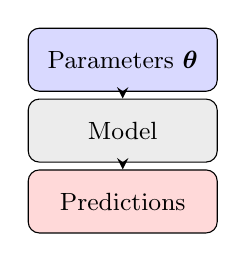
\begin{tikzpicture}[scale=0.75]
				\node[pipelinebox=blue!15, minimum width=2.4cm] (p) at (0,0) {Parameters $\boldsymbol{\theta}$};
				\node[pipelinebox=gray!15, minimum width=2.4cm] (m) at (0,-1.2) {Model};
				\node[pipelinebox=red!15, minimum width=2.4cm] (d) at (0,-2.4) {Predictions};
				\draw[pipelinearr] (p) -- (m);
				\draw[pipelinearr] (m) -- (d);
			\end{tikzpicture}\\[4pt]
			{\small \textit{``Given $\theta$, what does the cell do?''}}
		\end{column}
		\begin{column}{0.48\textwidth}
			\centering
			\textbf{Inference}\\[6pt]
			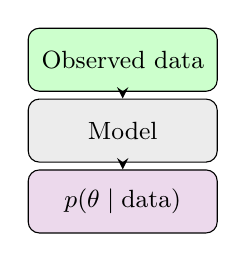
\begin{tikzpicture}[scale=0.75]
				\node[pipelinebox=green!20, minimum width=2.4cm] (d) at (0,0) {Observed data};
				\node[pipelinebox=gray!15, minimum width=2.4cm] (m) at (0,-1.2) {Model};
				\node[pipelinebox=colPost, minimum width=2.4cm] (p) at (0,-2.4) {$p(\theta \mid \text{data})$};
				\draw[pipelinearr] (d) -- (m);
				\draw[pipelinearr] (m) -- (p);
			\end{tikzpicture}\\[4pt]
			{\small \textit{``Given data, what $\theta$ are consistent?''}}
		\end{column}
	\end{columns}
\end{frame}




% SPEAKER NOTES:
% - The gap is semantic: the architecture has no representation for
%   probability. You cannot bolt a likelihood onto a system that stores
%   parameters as floats without rewriting the data structures.
% - Adding ABC on top of MC4D doesn't fix this: you can sample, but the
%   model itself still has no probabilistic semantics. Module boundaries
%   carry no distribution -- only point values.
% - InferCell makes parameters distributions natively, so every module
%   boundary can carry uncertainty by construction.
% - The runtime / polyglot side of the problem is set up *after* the
%   scientific payoff slide, as a feasibility gap -- see
%   "Why Pure Julia?" in the Architecture section.
%   Don't preview it here.



% ----------------------------------------------------------------
%\begin{frame}{What Inference Enables}
%
%	Inference lets you ask scientific questions that forward simulation cannot pose.
%
%	\bigskip
%	\begin{columns}[T]
%		\begin{column}{0.58\textwidth}
%			\begin{enumerate}\itemsep8pt
%				\item \textbf{Know which predictions to trust.}\\
%				{\small UQ. Probabilistic prediction. \\ \textit{"Is this prediction robust, or does it depend on parameter choices we're not confident about?"} }
%
%				\item \textbf{Learn biology from data.}\\
%				{\small Which parameters are identifiable? Does the modelling formalism matter (ODE vs SSA)? What should we measure next?}
%
%				\item \textbf{Discover when your model is wrong.}\\
%				{\small Posteriors far from literature values, or formalisms that disagree $\implies$ misspecification}
%			\end{enumerate}
%		\end{column}
%		\begin{column}{0.38\textwidth}
%			\centering
%			% 1. Predictions with uncertainty
%			\begin{tikzpicture}[scale=0.55]
%				\draw[->] (0,0) -- (4.2,0) node[right, font=\scriptsize] {$t$};
%				\draw[->] (0,0) -- (0,2.6);
%				\fill[violet!12] plot[smooth, domain=0:4] (\x, {1.8*(1-exp(-0.7*\x)) + 0.4})
%					-- plot[smooth, domain=4:0] (\x, {1.8*(1-exp(-0.7*\x)) - 0.4}) -- cycle;
%				\draw[thin, violet!40] plot[smooth, domain=0:4] (\x, {1.9*(1-exp(-0.65*\x)) + 0.15});
%				\draw[thin, violet!40] plot[smooth, domain=0:4] (\x, {1.7*(1-exp(-0.75*\x)) - 0.1});
%				\draw[thick, colPostLine] plot[smooth, domain=0:4] (\x, {1.8*(1-exp(-0.7*\x))});
%				\node[font=\scriptsize, colPostLine, anchor=west] at (2.5,2.3) {95\% CI};
%			\end{tikzpicture}
%
%			\vspace{6pt}
%
%			% 2. Identifiability: posterior vs prior
%			\begin{tikzpicture}[scale=0.55]
%				\draw[->] (0,0) -- (4,0) node[right, font=\scriptsize] {$\theta$};
%				\draw[->] (0,0) -- (0,2.4);
%				% Broad prior
%				\fill[gray!10] plot[smooth, domain=0.2:3.8] (\x, {0.7*exp(-0.2*(\x-2)^2)}) -- (3.8,0) -- (0.2,0) -- cycle;
%				\draw[thick, gray!50] plot[smooth, domain=0.2:3.8] (\x, {0.7*exp(-0.2*(\x-2)^2)});
%				% Tight posterior
%				\fill[colPost] plot[smooth, domain=0.3:3.7] (\x, {2.2*exp(-1.5*(\x-2.1)^2)}) -- (3.7,0) -- (0.3,0) -- cycle;
%				\draw[thick, colPostLine] plot[smooth, domain=0.3:3.7] (\x, {2.2*exp(-1.5*(\x-2.1)^2)});
%				\node[font=\scriptsize, gray!60, anchor=west] at (3.5,0.8) {prior};
%				\node[font=\scriptsize, colPostLine, anchor=west] at (3.5,1.8) {posterior};
%			\end{tikzpicture}
%
%			\vspace{6pt}
%
%			% 3. Model criticism: two formalisms disagree
%			\begin{tikzpicture}[scale=0.55]
%				\draw[->] (0,0) -- (4.2,0) node[right, font=\scriptsize] {$\theta$};
%				\draw[->] (0,0) -- (0,2.2);
%				\fill[blue!10] plot[smooth, domain=0.3:3.2] (\x, {1.8*exp(-1.8*(\x-1.4)^2)}) -- (3.2,0) -- (0.3,0) -- cycle;
%				\draw[thick, colODELine] plot[smooth, domain=0.3:3.2] (\x, {1.8*exp(-1.8*(\x-1.4)^2)});
%				\fill[orange!10] plot[smooth, domain=1.0:4.0] (\x, {1.6*exp(-1.5*(\x-2.8)^2)}) -- (4.0,0) -- (1.0,0) -- cycle;
%				\draw[thick, colSimLine] plot[smooth, domain=1.0:4.0] (\x, {1.6*exp(-1.5*(\x-2.8)^2)});
%				\node[font=\scriptsize, colODELine] at (0.7,1.9) {ODE};
%				\node[font=\scriptsize, colSimLine] at (3.6,1.7) {SSA};
%				\node[font=\scriptsize\itshape, colWarnLine, anchor=north] at (2.1,-0.3) {disagree $\Rightarrow$ formalism matters};
%			\end{tikzpicture}
%		\end{column}
%	\end{columns}
%\end{frame}
%


%\begin{frame}{What Inference Enables}
%	
%	Inference lets you ask scientific questions that forward simulation cannot pose.
%	
%	\bigskip
%	\begin{columns}[T]
%		\begin{column}{0.58\textwidth}
%			\begin{enumerate}\itemsep8pt
%				\item \textbf{Know which predictions to trust.}\\
%				{\small UQ. \textit{"Is this prediction robust, or does it depend on parameter choices we're not confident about?"} }
%				\item \textbf{Learn biology from data.}\\
%				{\small Identifiability, model selection, Bayesian OED. \\ \textit{``What can we actually learn from the data we have, and what should we measure next?"}}
%				\item \textbf{Discover when your model is wrong.}\\
%				{\small Posteriors far from literature values, or formalisms that disagree $\implies$ misspecification \\ \textit{"Where does our model break down?"} }
%			\end{enumerate}
%		\end{column}
%		\begin{column}{0.38\textwidth}
%			\centering
%			% 1. Predictions with uncertainty
%			\begin{tikzpicture}[scale=0.55]
%				\draw[->] (0,0) -- (4.2,0) node[right, font=\scriptsize] {$t$};
%				\draw[->] (0,0) -- (0,2.6);
%				\fill[violet!12] plot[smooth, domain=0:4] (\x, {1.8*(1-exp(-0.7*\x)) + 0.4})
%				-- plot[smooth, domain=4:0] (\x, {1.8*(1-exp(-0.7*\x)) - 0.4}) -- cycle;
%				\draw[thin, violet!40] plot[smooth, domain=0:4] (\x, {1.9*(1-exp(-0.65*\x)) + 0.15});
%				\draw[thin, violet!40] plot[smooth, domain=0:4] (\x, {1.7*(1-exp(-0.75*\x)) - 0.1});
%				\draw[thick, colPostLine] plot[smooth, domain=0:4] (\x, {1.8*(1-exp(-0.7*\x))});
%				\node[font=\scriptsize, colPostLine, anchor=west] at (2.5,2.3) {95\% CI};
%			\end{tikzpicture}
%			
%			\vspace{6pt}
%			
%			% 2. Identifiability: posterior vs prior
%			\begin{tikzpicture}[scale=0.55]
%				\draw[->] (0,0) -- (4,0) node[right, font=\scriptsize] {$\theta$};
%				\draw[->] (0,0) -- (0,2.4);
%				% Broad prior
%				\fill[gray!10] plot[smooth, domain=0.2:3.8] (\x, {0.7*exp(-0.2*(\x-2)^2)}) -- (3.8,0) -- (0.2,0) -- cycle;
%				\draw[thick, gray!50] plot[smooth, domain=0.2:3.8] (\x, {0.7*exp(-0.2*(\x-2)^2)});
%				% Tight posterior
%				\fill[colPost] plot[smooth, domain=0.3:3.7] (\x, {2.2*exp(-1.5*(\x-2.1)^2)}) -- (3.7,0) -- (0.3,0) -- cycle;
%				\draw[thick, colPostLine] plot[smooth, domain=0.3:3.7] (\x, {2.2*exp(-1.5*(\x-2.1)^2)});
%				\node[font=\scriptsize, gray!60, anchor=west] at (3.5,0.8) {prior};
%				\node[font=\scriptsize, colPostLine, anchor=west] at (3.5,1.8) {posterior};
%			\end{tikzpicture}
%			
%			\vspace{6pt}
%			
%			% 3. Model criticism: two formalisms disagree
%			\begin{tikzpicture}[scale=0.55]
%				\draw[->] (0,0) -- (4.2,0) node[right, font=\scriptsize] {$\theta$};
%				\draw[->] (0,0) -- (0,2.2);
%				\fill[blue!10] plot[smooth, domain=0.3:3.2] (\x, {1.8*exp(-1.8*(\x-1.4)^2)}) -- (3.2,0) -- (0.3,0) -- cycle;
%				\draw[thick, colODELine] plot[smooth, domain=0.3:3.2] (\x, {1.8*exp(-1.8*(\x-1.4)^2)});
%				\fill[orange!10] plot[smooth, domain=1.0:4.0] (\x, {1.6*exp(-1.5*(\x-2.8)^2)}) -- (4.0,0) -- (1.0,0) -- cycle;
%				\draw[thick, colSimLine] plot[smooth, domain=1.0:4.0] (\x, {1.6*exp(-1.5*(\x-2.8)^2)});
%				\node[font=\scriptsize, colODELine] at (0.7,1.9) {ODE};
%				\node[font=\scriptsize, colSimLine] at (3.6,1.7) {SSA};
%				\node[font=\scriptsize\itshape, colWarnLine, anchor=north] at (2.1,-0.3) {disagree $\Rightarrow$ formalism matters};
%			\end{tikzpicture}
%		\end{column}
%	\end{columns}
%\end{frame}




% ================================================================
% SECTION 3: Architecture
% ================================================================
\section{Architecture}


\begin{frame}{InferCell: Design Principles}
\alert{InferCell} is a composable, inference-first whole-cell modelling framework in Julia.
	\begin{columns}[T]
		\begin{column}{0.55\textwidth}
			\begin{itemize}\itemsep7pt
				\item \textbf{Inference-first.}\\
				{\small UQ and probabilistic prediction built in, not bolted on.}
				
				\item \textbf{Modular.}\\
				{\small Swap modules; inference still works.}
				
				\item \textbf{Information flow as design test.}\\
				{\small Every boundary: ``how does inference cross this?''}
				
				\item \textbf{Pure Julia.}\\
				{\small One language, one computational graph, no barriers to AD.}
			\end{itemize}
		\end{column}
		\begin{column}{0.42\textwidth}
			\centering
			% Modular: swap modules
			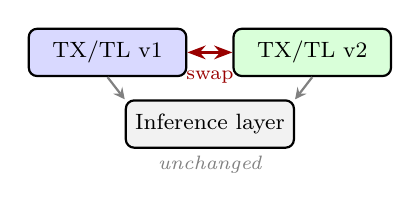
\begin{tikzpicture}[
				scale=0.65,
				mod/.style={draw, thick, rounded corners=3pt, minimum height=0.6cm, minimum width=2cm, align=center, font=\footnotesize},
				>=Stealth
				]
				\node[mod, fill=blue!15] (a) at (0,0) {TX/TL v1};
				\node[mod, fill=green!15] (b) at (4,0) {TX/TL v2};
				\draw[<->, thick, red!60!black] (a) -- (b) node[midway, below=3pt, font=\scriptsize] {swap};
				\node[mod, fill=gray!10] (inf) at (2,-1.4) {Inference layer};
				\draw[pipelinearr, gray] (a.south) -- (inf.north west);
				\draw[pipelinearr, gray] (b.south) -- (inf.north east);
				\node[font=\scriptsize\itshape, text=gray] at (2,-2.2) {unchanged};
			\end{tikzpicture}
			
			\vspace{10pt}
			
			% Information flow: module boundary with ?
			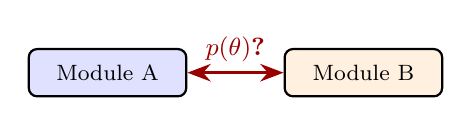
\begin{tikzpicture}[
				scale=0.65,
				mod/.style={draw, thick, rounded corners=3pt, minimum height=0.6cm, minimum width=2cm, align=center, font=\footnotesize},
				>=Stealth
				]
				\node[mod, fill=blue!12] (a) at (0,0) {Module A};
				\node[mod, fill=orange!12] (b) at (5,0) {Module B};
				\draw[<->, very thick, red!60!black] (a) -- (b) node[midway, above, font=\small\bfseries] {$p(\theta)$?};
			\end{tikzpicture}
			
			\vspace{10pt}
			
			% Pure Julia: single stack
			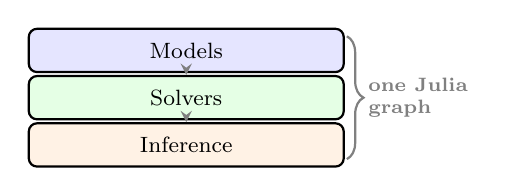
\begin{tikzpicture}[
				scale=0.6,
				layer/.style={draw, thick, rounded corners=3pt, minimum height=0.55cm, minimum width=4cm, align=center, font=\footnotesize},
				>=Stealth
				]
				\node[layer, fill=blue!10] (mod) at (0,1.8) {Models};
				\node[layer, fill=green!10] (sol) at (0,0.8) {Solvers};
				\node[layer, fill=orange!10] (inf) at (0,-0.2) {Inference};
				\draw[pipelinearr, gray] (mod) -- (sol);
				\draw[pipelinearr, gray] (sol) -- (inf);
				\draw[brace, thick, gray] (3.4,2.1) -- (3.4,-0.5)
				node[midway, right=4pt, font=\scriptsize\bfseries, text=gray, align=left] {one Julia\\graph};
			\end{tikzpicture}
		\end{column}
	\end{columns}
\end{frame}


%% ----------------------------------------------------------------
%\begin{frame}{What Becomes Possible}
%	\scriptsize
%	Scientific questions that forward simulation cannot pose:
%	
%	\medskip
%	\begin{columns}[T]
%		\begin{column}{0.48\textwidth}
%			\textbf{Quantitative biology}
%			\begin{itemize}\itemsep0pt\parskip0pt
%				\item Which parameters does the data actually constrain?
%				\item Is mechanism $X$ consistent with the observations?
%				\item Are competing hypotheses distinguishable?
%				\item Where does the model fail to reproduce reality?
%			\end{itemize}
%			
%			\medskip
%			\textbf{Structural inference}
%			\begin{itemize}\itemsep0pt\parskip0pt
%				\item Discover which reactions are present, from data
%				\item Recover dynamically-equivalent CRN families
%				\item Quantify structural uncertainty alongside parameters
%			\end{itemize}
%		\end{column}
%		\begin{column}{0.48\textwidth}
%			\textbf{Experimental design}
%			\begin{itemize}\itemsep0pt\parskip0pt
%				\item What should I measure next?
%				\item Which experiment maximises information gain?
%				\item What's the value of a new dataset before running it?
%				\item How does information propagate between subsystems?
%			\end{itemize}
%			
%			\medskip
%			\textbf{Model criticism}
%			\begin{itemize}\itemsep0pt\parskip0pt
%				\item Posterior predictive checks for misspecification
%				\item Compare formalisms (ODE vs SSA) on the same data
%				\item Detect when literature priors conflict with observations
%			\end{itemize}
%		\end{column}
%	\end{columns}
%	
%	\vfill
%	\centering
%	\alert{Forward simulation never reveals these. The framework is what makes them rigorous.}
%\end{frame}


\begin{frame}{What Becomes Possible}
	\small
	Scientific questions that forward simulation cannot pose:

	\medskip
	\begin{columns}[T]
		\begin{column}{0.48\textwidth}
			\textbf{Probabilistic predictions}
			\begin{itemize}\itemsep0pt\parskip0pt
				\item Credible intervals on observables
			\end{itemize}

			\medskip
			\textbf{Inference from data}
			\begin{itemize}\itemsep0pt\parskip0pt
				\item Bayesian calibration + updating
			\end{itemize}

			\medskip
			\textbf{Identifiability}
			\begin{itemize}\itemsep0pt\parskip0pt
				\item Which parameters does the data constrain?
			\end{itemize}
		\end{column}
		\begin{column}{0.48\textwidth}
			\textbf{Model criticism}
			\begin{itemize}\itemsep0pt\parskip0pt
				\item Posterior predictive checks; Bayes factors
			\end{itemize}

			\medskip
			\textbf{Experimental design}
			\begin{itemize}\itemsep0pt\parskip0pt
				\item Expected information gain
			\end{itemize}

			\medskip
			\textbf{Biology discovery}
			\begin{itemize}\itemsep0pt\parskip0pt
				\item Is mechanism $X$ consistent with the data?
			\end{itemize}
		\end{column}
	\end{columns}
\end{frame}


% ----------------------------------------------------------------
\begin{frame}{Why Pure Julia?}
	\begin{columns}[T]
		\begin{column}{0.55\textwidth}
			\textbf{Standard WCMs are polyglot stacks.}
			\begin{itemize}\itemsep5pt
				\item Python $+$ C++ $+$ CUDA $+$ LAMMPS, glued by IO
				\item Module boundaries are crossed by serialization, not by reference
				\item Gradients don't compose across language boundaries
			\end{itemize}
			
						\textbf{\footnotesize InferCell: one Julia stack}
			\begin{itemize}\itemsep1pt\footnotesize
				\item DifferentialEquations.jl --- solvers
				\item Turing.jl --- Bayesian inference
				\item SciMLSensitivity.jl --- AD through solvers
				\item Catalyst.jl --- reaction networks
			\end{itemize}
			
			
		\end{column}
		\begin{column}{0.42\textwidth}
			\centering
			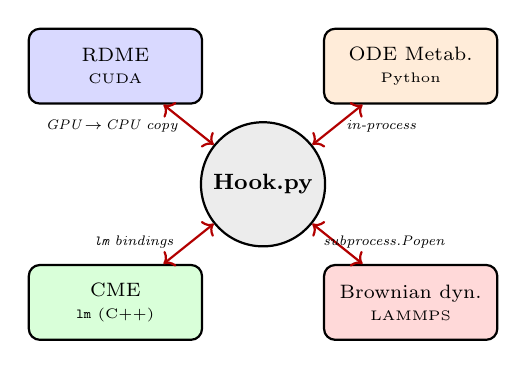
\begin{tikzpicture}[
				scale=0.5,
				every node/.style={font=\scriptsize},
				iolabel/.style={font=\tiny\itshape, black}
			]
				\node[draw, rounded corners=4pt, thick, fill=blue!15,
				      minimum height=0.95cm, minimum width=2.2cm, align=center]
				     (rdme) at (-2,5) {RDME\\\tiny CUDA};
				\node[draw, rounded corners=4pt, thick, fill=orange!15,
				      minimum height=0.95cm, minimum width=2.2cm, align=center]
				     (ode) at (5.5,5) {ODE Metab.\\\tiny Python};
				\node[draw, rounded corners=4pt, thick, fill=green!15,
				      minimum height=0.95cm, minimum width=2.2cm, align=center]
				     (cme) at (-2,-1) {CME\\\tiny \texttt{lm} (C++)};
				\node[draw, rounded corners=4pt, thick, fill=red!15,
				      minimum height=0.95cm, minimum width=2.2cm, align=center]
				     (bd) at (5.5,-1) {Brownian dyn.\\\tiny LAMMPS};
				\node[draw, circle, thick, fill=gray!15, minimum size=1.1cm, align=center]
				     (sim) at (1.75,2) {\textbf{\footnotesize Hook.py}};
				\draw[<->, thick, colWarnLine] (rdme) -- node[iolabel, above, pos=0.4, yshift=-8pt, xshift=-26pt]
				     {GPU\,$\to$\,CPU copy} (sim);
				\draw[<->, thick, colWarnLine] (ode) -- node[iolabel, above, pos=0.4, yshift=-8pt, xshift=14pt]
				     {in-process} (sim);
				\draw[<->, thick, colWarnLine] (cme) -- node[iolabel, below, pos=0.4, yshift=8pt, xshift=-18pt]
				     {\texttt{lm} bindings} (sim);
				\draw[<->, thick, colWarnLine] (bd) -- node[iolabel, below, pos=0.4, yshift=8pt, xshift=15pt]
				     {subprocess.Popen} (sim);
			\end{tikzpicture}

		\end{column}
	\end{columns}


\end{frame}


% ----------------------------------------------------------------
\begin{frame}{What Becomes Possible (Engineering)}
	\small
	Engineering capabilities that a single compiled runtime unlocks:

	\medskip
	\begin{columns}[T]
		\begin{column}{0.48\textwidth}
			\textbf{Performance \& HPC}
			\begin{itemize}\itemsep0pt\parskip0pt
				\item Whole model as one program; profile and run as a single GPU pipeline
			\end{itemize}

			\medskip
			\textbf{End-to-end gradients}
			\begin{itemize}\itemsep0pt\parskip0pt
				\item AD through solvers, models, and inference --- HMC/NUTS, VI, gradient-based BOED at WCM scale
			\end{itemize}

			\medskip
			\textbf{Hybrid inference}
			\begin{itemize}\itemsep0pt\parskip0pt
				\item NUTS and SBI blocks compose; boundary protocol lives in the type system
			\end{itemize}
		\end{column}
		\begin{column}{0.48\textwidth}
			\textbf{Composability \& substitution}
			\begin{itemize}\itemsep0pt\parskip0pt
				\item Swap solvers (ODE $\leftrightarrow$ SSA), drop in ML surrogates --- no cross-language plumbing
			\end{itemize}

			\medskip
			\textbf{Shared infrastructure}
			\begin{itemize}\itemsep0pt\parskip0pt
				\item One type system, one dependency stack, uniform logging and stack traces
			\end{itemize}

			\medskip
			\textbf{Cheap prototyping}
			\begin{itemize}\itemsep0pt\parskip0pt
				\item Add a module without committing to its language's ecosystem
			\end{itemize}
		\end{column}
	\end{columns}
\end{frame}




% ----------------------------------------------------------------
\begin{frame}{Hybrid Inference}
	Cells mix fundamentally different dynamics in the same model:

	\bigskip
	\begin{columns}[T]
		\begin{column}{0.48\textwidth}
			\centering
			\textbf{Differentiable dynamics}\\[4pt]
			{\small ODE metabolism, continuous kinetics}\\[8pt]
			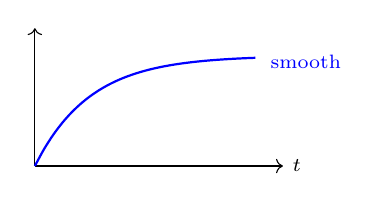
\begin{tikzpicture}[scale=0.7]
				\draw[->] (0,0) -- (4.5,0) node[right, font=\scriptsize] {$t$};
				\draw[->] (0,0) -- (0,2.5);
				\draw[thick, blue] plot[smooth, domain=0:4] (\x, {2*(1-exp(-\x))});
				\node[font=\scriptsize, blue, anchor=west] at (4.1,1.9) {smooth};
			\end{tikzpicture}\\[4pt]
			$\to$ Gradients exist\\
			$\to$ \textbf{NUTS / HMC}\\[3pt]
			{\scriptsize\itshape Orders of magnitude more efficient}
		\end{column}
		\begin{column}{0.48\textwidth}
			\centering
			\textbf{Stochastic dynamics}\\[4pt]
			{\small Gillespie SSA, gene switching}\\[8pt]
			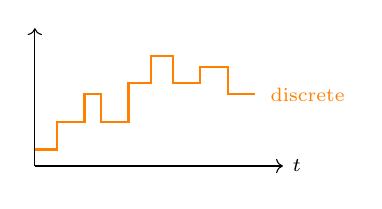
\begin{tikzpicture}[scale=0.7]
				\draw[->] (0,0) -- (4.5,0) node[right, font=\scriptsize] {$t$};
				\draw[->] (0,0) -- (0,2.5);
				\draw[thick, orange] (0,0.3) -- (0.4,0.3) -- (0.4,0.8) -- (0.9,0.8)
					-- (0.9,1.3) -- (1.2,1.3) -- (1.2,0.8) -- (1.7,0.8)
					-- (1.7,1.5) -- (2.1,1.5) -- (2.1,2.0) -- (2.5,2.0)
					-- (2.5,1.5) -- (3.0,1.5) -- (3.0,1.8) -- (3.5,1.8)
					-- (3.5,1.3) -- (4.0,1.3);
				\node[font=\scriptsize, orange, anchor=west] at (4.1,1.3) {discrete};
			\end{tikzpicture}\\[4pt]
			$\to$ No gradient path\\
			$\to$ \textbf{SBI / ABC-SMC}\\[3pt]
			{\scriptsize\itshape Handles any simulator as black box}
		\end{column}
	\end{columns}

	\vspace{2mm}

	No single inference method handles both.\\The hybrid graph uses each method where it is strongest.
\end{frame}

% ----------------------------------------------------------------
\begin{frame}{The Inference Graph}
	\centering
	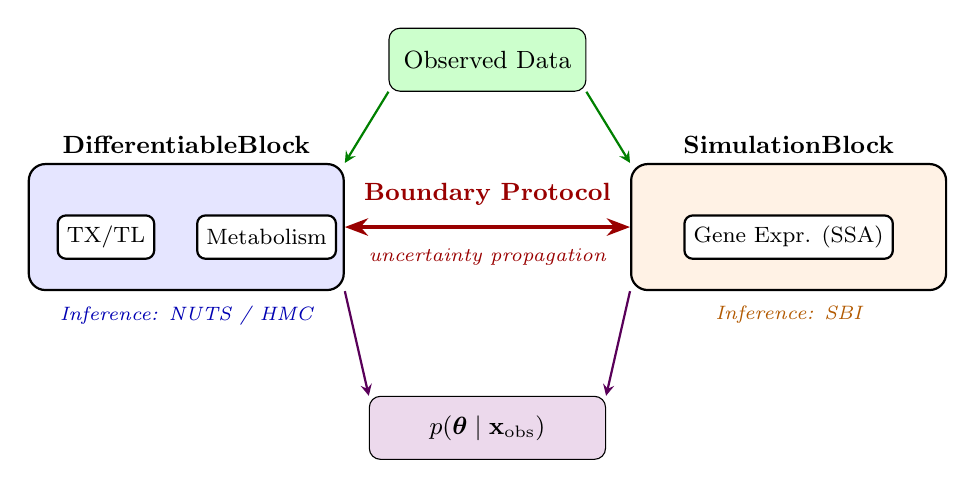
\begin{tikzpicture}[
		scale=0.85,
		block/.style={draw, thick, rounded corners=6pt, minimum height=1.6cm, minimum width=4cm, align=center},
		smallmod/.style={draw, rounded corners=3pt, minimum height=0.55cm, font=\footnotesize, fill=white, thick},
		>=Stealth
	]
		% Differentiable block
		\node[block, fill=blue!10] (diff) at (-0.5,0) {};
		\node[above, font=\small\bfseries] at (diff.north) {DifferentiableBlock};
		\node[smallmod] (tx) at (-1.7,-0.15) {TX/TL};
		\node[smallmod] (met) at (0.7,-0.15) {Metabolism};
		\node[below=2pt, font=\scriptsize\itshape, text=blue!70!black] at (diff.south) {Inference: NUTS / HMC};

		% Simulation block
		\node[block, fill=orange!10] (sim) at (8.5,0) {};
		\node[above, font=\small\bfseries] at (sim.north) {SimulationBlock};
		\node[smallmod] (ssa) at (8.5,-0.15) {Gene Expr. (SSA)};
		\node[below=2pt, font=\scriptsize\itshape, text=orange!70!black] at (sim.south) {Inference: SBI};

		% Boundary
		\draw[<->, very thick, red!60!black] (diff.east) -- (sim.west)
			node[midway, above=4pt, font=\small\bfseries] {Boundary Protocol}
			node[midway, below=4pt, font=\scriptsize\itshape] {uncertainty propagation};

		% Data arrow
		\node[pipelinebox=green!20, minimum width=2.5cm] (data) at (4,2.5) {Observed Data};
		\draw[pipelinearr, green!50!black] (data.south west) -- (diff.north east);
		\draw[pipelinearr, green!50!black] (data.south east) -- (sim.north west);

		% Posterior arrow
		\node[pipelinebox=colPost, minimum width=3cm] (post) at (4,-3) {$p(\boldsymbol{\theta} \mid \textbf{x}_\mathrm{obs})$};
		\draw[pipelinearr, colPostLine] (diff.south east) -- (post.north west);
		\draw[pipelinearr, colPostLine] (sim.south west) -- (post.north east);
	\end{tikzpicture}

	\medskip
	{\small Modules are automatically partitioned into blocks by their declared inference mode.}
\end{frame}




% ----------------------------------------------------------------
\begin{frame}{Conditioning the Whole Model}
	\centering
	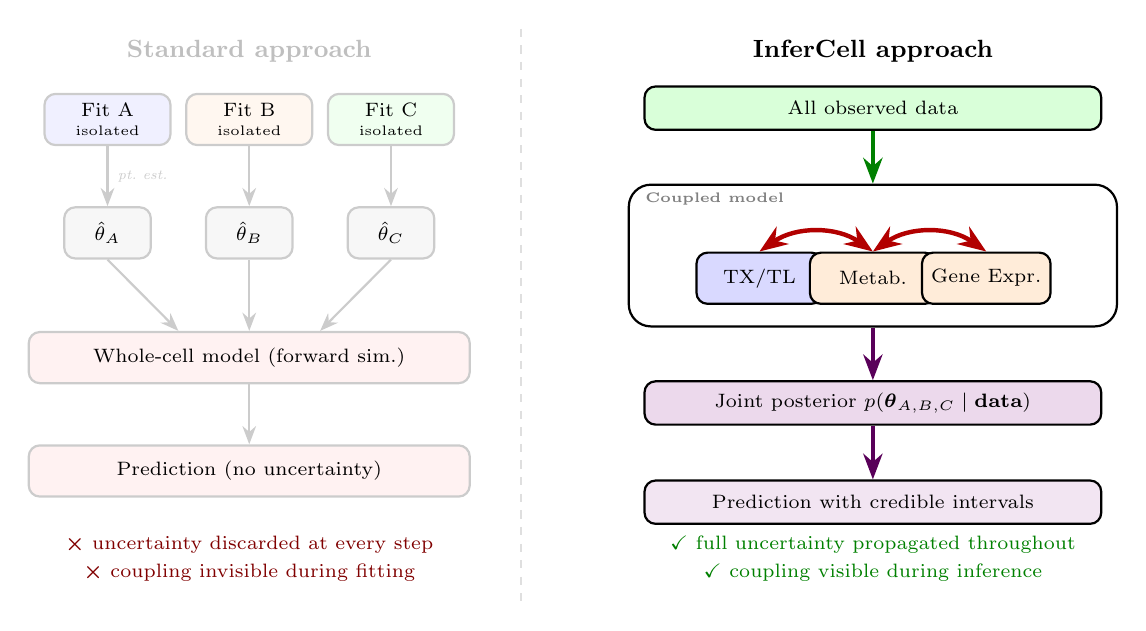
\begin{tikzpicture}[
		scale=0.72,
		mod/.style={draw, thick, rounded corners=4pt, minimum height=0.65cm, align=center, font=\scriptsize},
		>=Stealth
	]
		% ===== LEFT: Standard approach (dimmed) =====
		\node[font=\small\bfseries, text=gray!50] at (-5.5, 5.2) {Standard approach};

		% Isolated fits
		\node[mod, fill=blue!6, draw=gray!40, minimum width=1.6cm] (fA) at (-8, 4.0) {Fit A\\[-1pt]{\tiny isolated}};
		\node[mod, fill=orange!6, draw=gray!40, minimum width=1.6cm] (fB) at (-5.5, 4.0) {Fit B\\[-1pt]{\tiny isolated}};
		\node[mod, fill=green!6, draw=gray!40, minimum width=1.6cm] (fC) at (-3, 4.0) {Fit C\\[-1pt]{\tiny isolated}};

		% Point estimates
		\node[mod, fill=gray!6, draw=gray!40, minimum width=1.1cm] (pA) at (-8, 2.0) {$\hat{\theta}_A$};
		\node[mod, fill=gray!6, draw=gray!40, minimum width=1.1cm] (pB) at (-5.5, 2.0) {$\hat{\theta}_B$};
		\node[mod, fill=gray!6, draw=gray!40, minimum width=1.1cm] (pC) at (-3, 2.0) {$\hat{\theta}_C$};

		\draw[->, thick, gray!40] (fA) -- (pA) node[midway, right, font=\tiny\itshape, text=gray!40] {pt.\ est.};
		\draw[->, thick, gray!40] (fB) -- (pB);
		\draw[->, thick, gray!40] (fC) -- (pC);

		% Assembly
		\node[mod, fill=red!5, draw=gray!40, minimum width=5.6cm] (wcm) at (-5.5, -0.2) {Whole-cell model (forward sim.)};
		\draw[->, thick, gray!40] (pA.south) -- ([xshift=-1.25cm]wcm.north);
		\draw[->, thick, gray!40] (pB) -- (wcm);
		\draw[->, thick, gray!40] (pC.south) -- ([xshift=1.25cm]wcm.north);

		% Output
		\node[mod, fill=red!5, draw=gray!40, minimum width=5.6cm] (out) at (-5.5, -2.2) {Prediction (no uncertainty)};
		\draw[->, thick, gray!40] (wcm) -- (out);

		% Problems
		\node[font=\scriptsize, text=red!50!black] at (-5.5, -3.5) {$\boldsymbol{\times}$ uncertainty discarded at every step};
		\node[font=\scriptsize, text=red!50!black] at (-5.5, -4.0) {$\boldsymbol{\times}$ coupling invisible during fitting};

		% ===== DIVIDER =====
		\draw[thick, gray!25, dashed] (-0.7, 5.6) -- (-0.7, -4.5);

		% ===== RIGHT: InferCell (vivid) =====
		% Layout: equal gaps (~0.97 TikZ units) between all four block edges.
		% Box 1.8cm tall; three small boxes 0.55cm tall; scale=0.72.
		\node[font=\small\bfseries] at (5.5, 5.2) {InferCell approach};

		% Data at top
		\node[draw, thick, rounded corners=4pt, fill=green!15,
			  font=\scriptsize, minimum width=5.8cm, minimum height=0.55cm]
			  (data) at (5.5, 4.2) {All observed data};

		% Coupled model box
		\node[draw, thick, rounded corners=8pt,
			  minimum height=1.8cm, minimum width=6.2cm,
			  fill=white] (cbox) at (5.5, 1.6) {};
		\node[font=\tiny\bfseries, text=gray, anchor=north west]
			  at ([xshift=4pt]cbox.north west) {Coupled model};

		% Modules inside the box
		\node[mod, fill=blue!15, minimum width=1.6cm] (mA) at (3.5, 1.2) {TX/TL};
		\node[mod, fill=orange!15, minimum width=1.6cm] (mB) at (5.5, 1.2) {Metab.};
		\node[mod, fill=orange!15, minimum width=1.6cm] (mC) at (7.5, 1.2) {Gene Expr.};

		% Coupling arrows --- arched above the modules
		\draw[<->, line width=1.6pt, red!70!black] (mA.north) to[bend left=35] (mB.north);
		\draw[<->, line width=1.6pt, red!70!black] (mB.north) to[bend left=35] (mC.north);

		% Data -> coupled model
		\draw[->, line width=1.4pt, green!50!black] (data) -- (cbox);

		% Joint posterior
		\node[draw, thick, rounded corners=4pt, fill=colPost,
			  font=\scriptsize, minimum width=5.8cm, minimum height=0.55cm]
			  (post) at (5.5, -1.0) {Joint posterior $p(\boldsymbol{\theta}_{A,B,C} \mid \textbf{data})$};
		\draw[->, line width=1.4pt, colPostLine] (cbox) -- (post);

		% Prediction with UQ
		\node[draw, thick, rounded corners=4pt, fill=violet!10,
			  font=\scriptsize, minimum width=5.8cm, minimum height=0.55cm]
			  (predR) at (5.5, -2.75) {Prediction with credible intervals};
		\draw[->, line width=1.4pt, colPostLine] (post) -- (predR);

		% Benefits
		\node[font=\scriptsize, text=green!50!black] at (5.5, -3.5) {$\checkmark$ full uncertainty propagated throughout};
		\node[font=\scriptsize, text=green!50!black] at (5.5, -4.0) {$\checkmark$ coupling visible during inference};
	\end{tikzpicture}

\end{frame}

% ----------------------------------------------------------------
\begin{frame}{How Much Coupling Do You Need?}
Joint inference over all parameters is intractable. \newline  Isolated submodel fits discard all coupling. 

	\bigskip
	\centering
	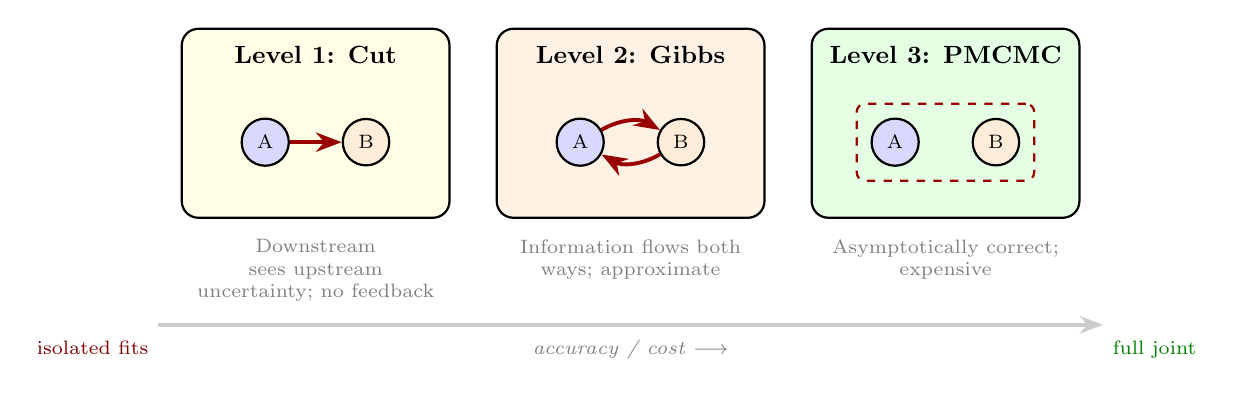
\begin{tikzpicture}[
		scale=0.8,
		lvl/.style={draw, thick, rounded corners=6pt, minimum height=2.4cm, minimum width=3.4cm, align=center},
		circ/.style={draw, thick, circle, minimum size=0.55cm, font=\scriptsize},
		>=Stealth
	]
		% Level 1: Cut
		\node[lvl, fill=yellow!10] (l1) at (0, 0) {};
		\node[font=\small\bfseries, anchor=north] at ([yshift=-4pt]l1.north) {Level 1: Cut};
		\node[circ, fill=blue!15] (a1) at (-0.8, -0.3) {A};
		\node[circ, fill=orange!15] (b1) at (0.8, -0.3) {B};
		\draw[->, line width=1.4pt, red!60!black] (a1) -- (b1);
		\node[font=\scriptsize, text=gray, text width=3.2cm, align=center, anchor=north]
			at ([yshift=-5pt]l1.south) {Downstream sees upstream\\uncertainty; no feedback};

		% Level 2: Gibbs
		\node[lvl, fill=orange!10] (l2) at (5, 0) {};
		\node[font=\small\bfseries, anchor=north] at ([yshift=-4pt]l2.north) {Level 2: Gibbs};
		\node[circ, fill=blue!15] (a2) at (4.2, -0.3) {A};
		\node[circ, fill=orange!15] (b2) at (5.8, -0.3) {B};
		\draw[->, line width=1.4pt, red!60!black] (a2) to[bend left=30] (b2);
		\draw[->, line width=1.4pt, red!60!black] (b2) to[bend left=30] (a2);
		\node[font=\scriptsize, text=gray, text width=3.2cm, align=center, anchor=north]
			at ([yshift=-5pt]l2.south) {Information flows both\\ways; approximate};

		% Level 3: PMCMC
		\node[lvl, fill=green!10] (l3) at (10, 0) {};
		\node[font=\small\bfseries, anchor=north] at ([yshift=-4pt]l3.north) {Level 3: PMCMC};
		\node[circ, fill=blue!15] (a3) at (9.2, -0.3) {A};
		\node[circ, fill=orange!15] (b3) at (10.8, -0.3) {B};
		\node[draw, thick, dashed, rounded corners=3pt, red!60!black,
			  inner sep=5pt, fit=(a3)(b3)] {};
		\node[font=\scriptsize, text=gray, text width=3.2cm, align=center, anchor=north]
			at ([yshift=-5pt]l3.south) {Asymptotically correct;\\expensive};

		% Progression arrow
		\draw[->, line width=1.2pt, gray!40] (-2.5, -3.2) -- (12.5, -3.2);
		\node[font=\scriptsize, text=red!50!black, anchor=north east] at (-2.5, -3.3) {isolated fits};
		\node[font=\scriptsize, text=green!50!black, anchor=north west] at (12.5, -3.3) {full joint};
		\node[font=\scriptsize\itshape, text=gray] at (5, -3.6) {accuracy / cost $\longrightarrow$};
	\end{tikzpicture}

%	\begin{itemize}\itemsep2pt
%		\item { The framework lets you \textbf{choose the level of inferential coupling} for the question you are asking}
%		\item {\tiny \textbf{Diagnostic:} does the posterior change when you allow feedback? If not, the cut was sufficient}
%	\end{itemize}
\end{frame}



% ================================================================
% SECTION 4: What This Looks Like in Practice
% ================================================================
\section{In Practice}




  \begin{frame}{Toy example: a 3-module WCM}
	\centering
	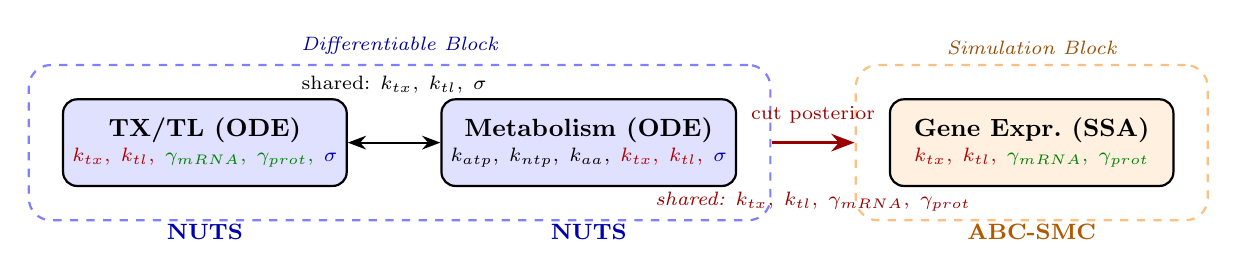
\begin{tikzpicture}[
		scale=0.75,
		mod/.style={draw, thick, rounded corners=5pt, minimum height=1.1cm, minimum width=3.6cm, align=center, font=\small},
		>=Stealth
		]
		% Modules — spread out for label clearance
		% Color code: red = shared across all 3 modules, green = shared across blocks (TX/TL + SSA),
		%             blue = shared within DifferentiableBlock only, black = unique
		\node[mod, fill=blue!12] (txl) at (0,0) {\textbf{TX/TL (ODE)}\\[-2pt]\scriptsize $\color{red!70!black}k_{tx},\; \color{red!70!black}k_{tl},\; \color{green!50!black}\gamma_{mRNA},\; \color{green!50!black}\gamma_{prot},\; \color{blue!70!black}\sigma$};
		\node[mod, fill=blue!12] (met) at (6.5,0) {\textbf{Metabolism (ODE)}\\[-2pt]\scriptsize $k_{atp},\; k_{ntp},\; k_{aa},\; \color{red!70!black}k_{tx},\; \color{red!70!black}k_{tl},\; \color{blue!70!black}\sigma$};
		\node[mod, fill=orange!12] (ssa) at (14,0) {\textbf{Gene Expr.\ (SSA)}\\[-2pt]\scriptsize $\color{red!70!black}k_{tx},\; \color{red!70!black}k_{tl},\; \color{green!50!black}\gamma_{mRNA},\; \color{green!50!black}\gamma_{prot}$};
		
		% Inference labels
		\node[below=10pt, font=\footnotesize\bfseries, text=blue!70!black] at (txl.south) {NUTS};
		\node[below=10pt, font=\footnotesize\bfseries, text=blue!70!black] at (met.south) {NUTS};
		\node[below=10pt, font=\footnotesize\bfseries, text=orange!70!black] at (ssa.south) {ABC-SMC};
		
		% Coupling arrows within ODE block
		\draw[<->, thick] (txl) -- (met) node[midway, above=14pt, font=\scriptsize] {shared: $k_{tx},\; k_{tl},\; \sigma$};
		
		% Block grouping
		\node[draw, dashed, thick, blue!50, rounded corners=8pt, fit=(txl)(met), inner sep=12pt, label={[font=\scriptsize\itshape, text=blue!60!black]above:Differentiable Block}] (diffblock) {};
		\node[draw, dashed, thick, orange!50, rounded corners=8pt, fit=(ssa), inner sep=12pt, label={[font=\scriptsize\itshape, text=orange!60!black]above:Simulation Block}] (simblock) {};
		
		% Boundary: unidirectional from ODE block to SSA (cut posterior)
		\draw[->, very thick, red!60!black] (diffblock.east) -- (simblock.west)
		node[midway, above=3pt, font=\scriptsize] {cut posterior}
		node[midway, below=14pt, font=\scriptsize\itshape] {shared: $k_{tx},\; k_{tl},\; \gamma_{mRNA},\; \gamma_{prot}$};
	\end{tikzpicture}
	
	\bigskip
	\begin{itemize}\itemsep4pt
		\item Same biology (TX/TL) modelled as ODE and SSA $\to$ direct comparison of posteriors across formalisms
		\item ${\sim}$9 unique parameters after deduplication (shared across modules), all with priors
		\item Validated on synthetic data where ground truth is known
	\end{itemize}
\end{frame}

% ----------------------------------------------------------------
\begin{frame}{Joint parameter estimation}
	\centering
	
\includegraphics[width=0.48\textwidth]{figures/step3_corner.png}
	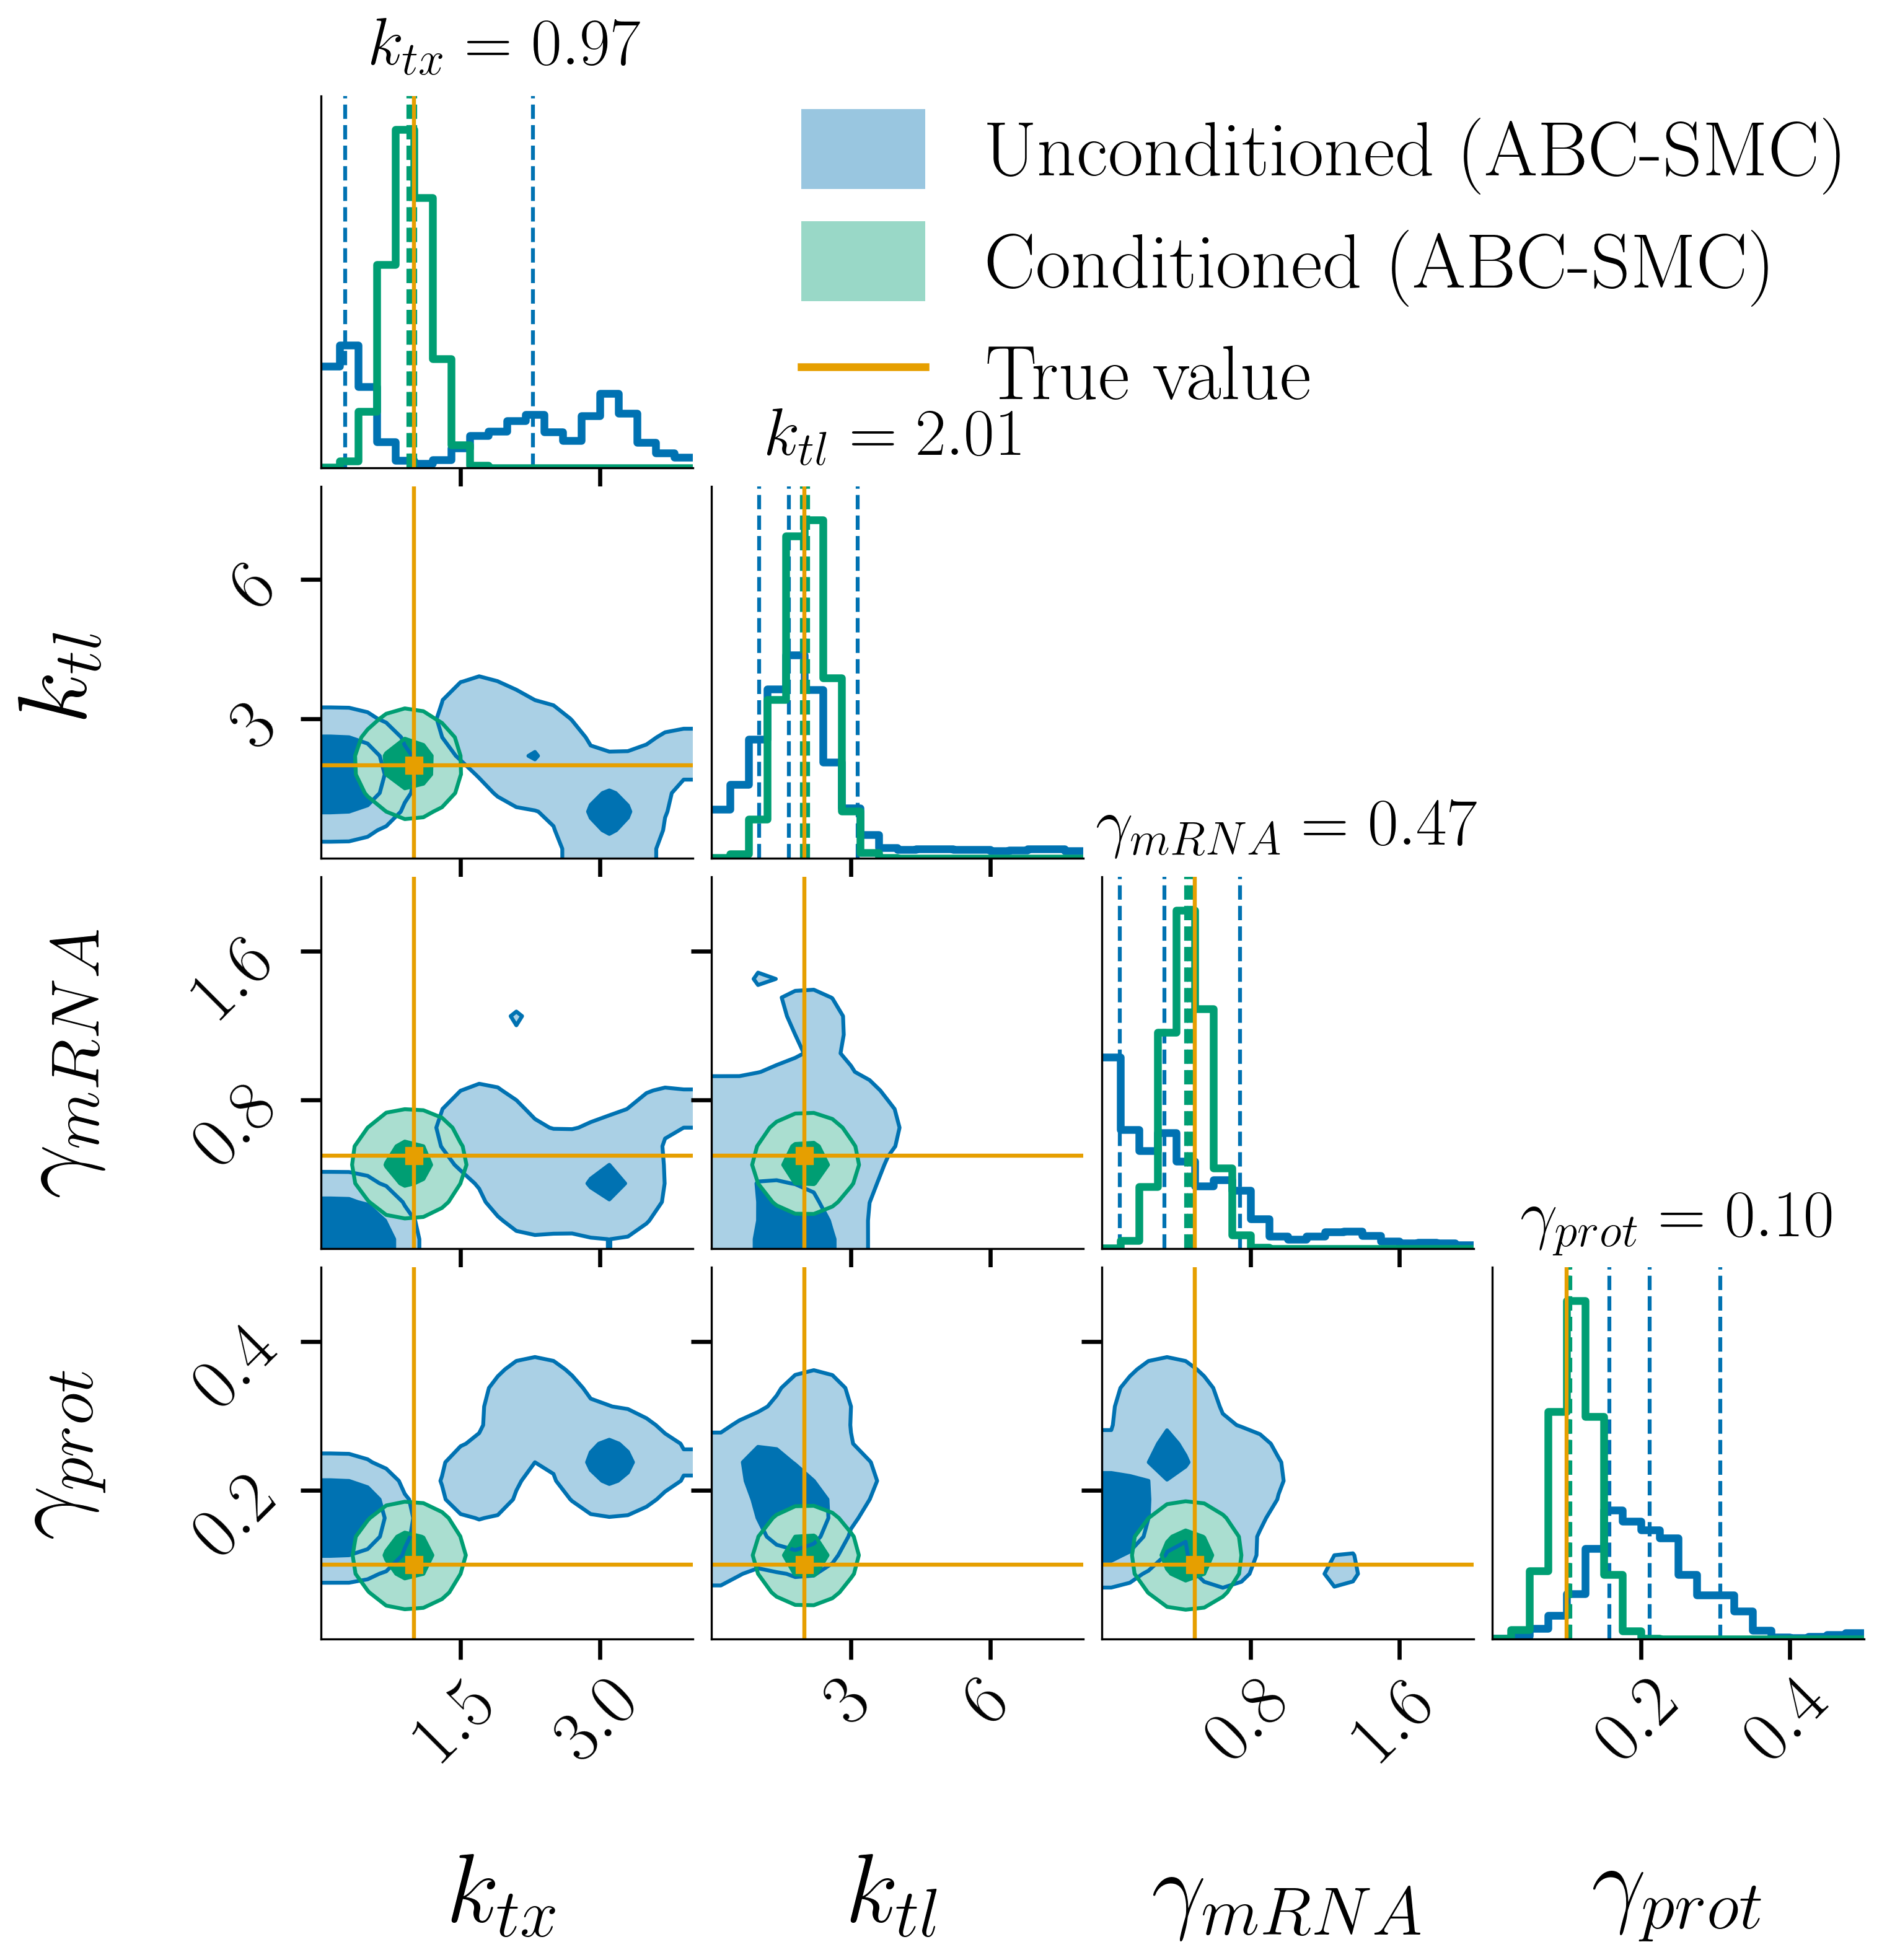
\includegraphics[width=0.48\textwidth]{figures/step3_ssa_posteriors.png}
\end{frame}



\begin{frame}{Level-2 Iterative Boundary: Posterior Tightening}
	\begin{columns}[T]
		\begin{column}{0.55\textwidth}
			\centering
			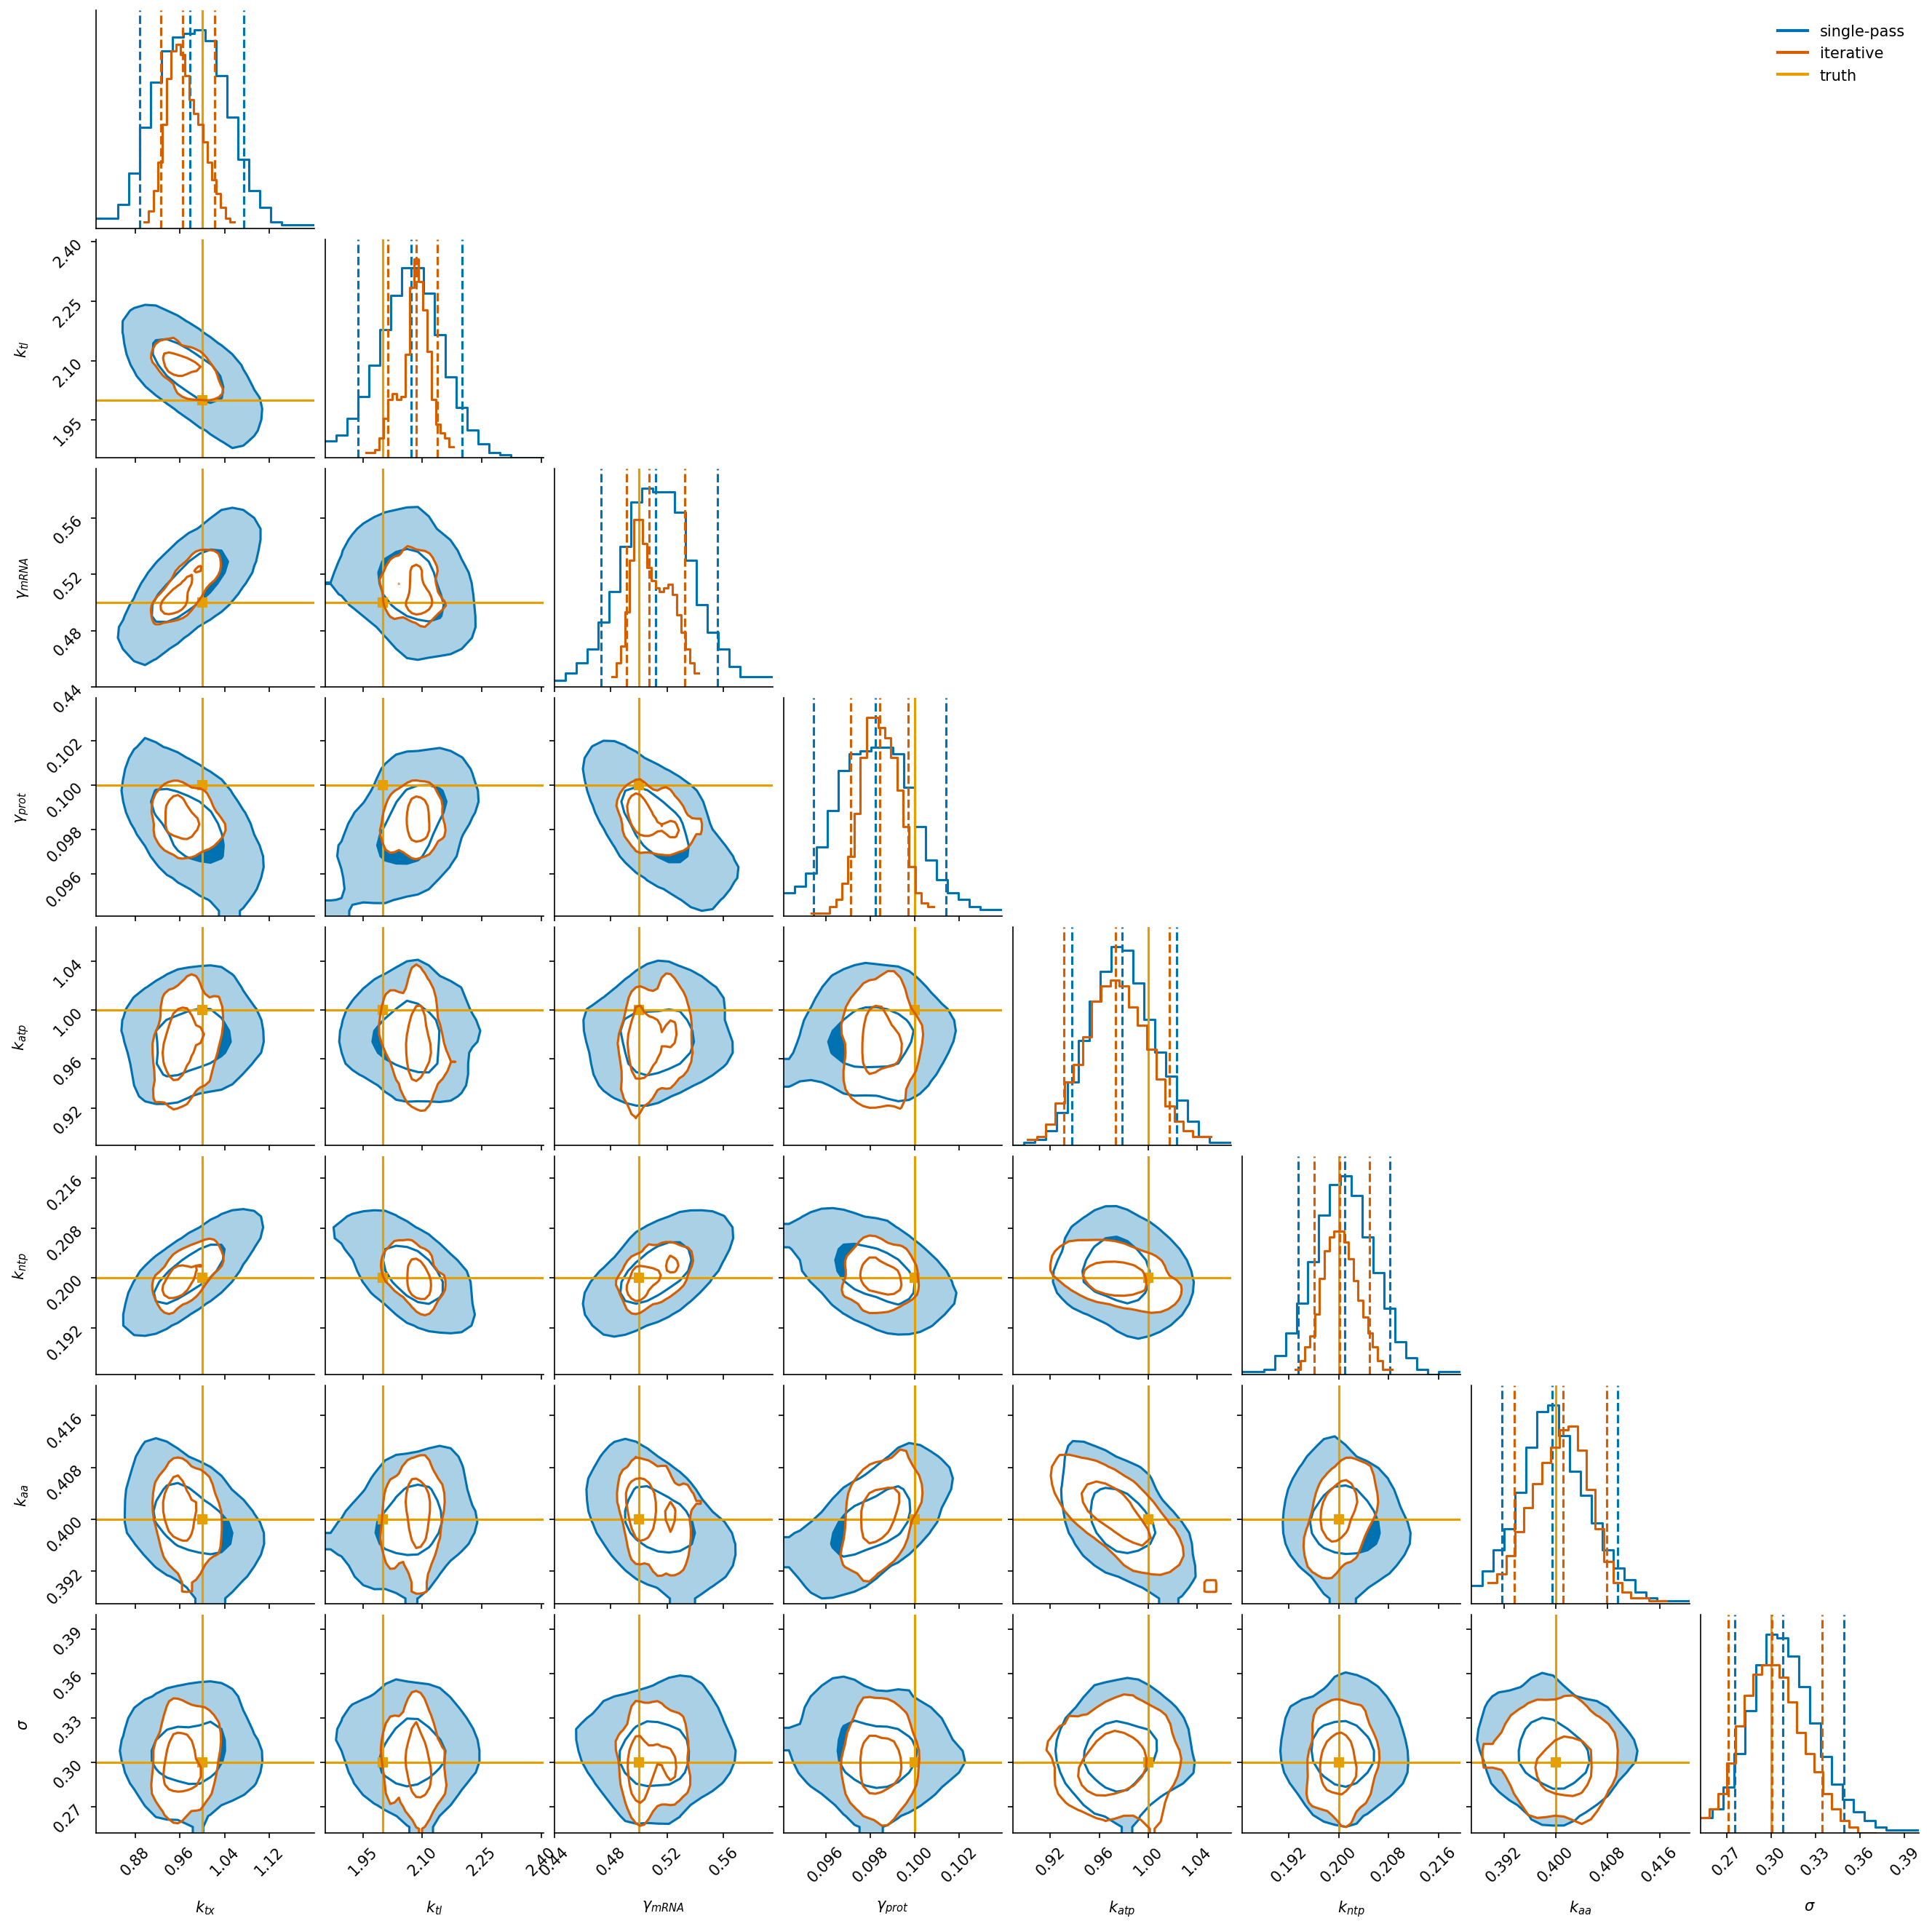
\includegraphics[width=0.95\textwidth]{figures/step4_corner.png}\\[3pt]
			{\scriptsize\itshape Single-pass (blue) vs Level-2 iterative (orange) posteriors; truth in yellow.}
		\end{column}
		\begin{column}{0.42\textwidth}
			\footnotesize
			\textbf{Closed-loop synthetic biology}
			\begin{itemize}\itemsep3pt
				\item ODE block: TX/TL $+$ enzyme-feedback metabolism
				\item SSA block: bursty (telegraph) regulator
				\item Shared params: $k_{tl},\;\gamma_{mRNA},\;\gamma_{prot}$
			\end{itemize}
			
			\medskip
			\textbf{90\% CI width on shared params}\\[2pt]
			\begin{tabular}{lrrr}
				\toprule
				& single & iter & $\Delta$ \\
				\midrule
				$k_{tl}$        & 0.264 & 0.125 & $-53\%$ \\
				$\gamma_{mRNA}$ & 0.083 & 0.041 & $-51\%$ \\
				$\gamma_{prot}$ & 0.006 & 0.003 & $-50\%$ \\
				\bottomrule
			\end{tabular}
		\end{column}
	\end{columns}
	
	\vfill
	{\scriptsize\itshape Single-pass 95\% CI covers truth on 4/4 ODE params; iter 95\% covers 2/4, iter 99\% covers 4/4 --- mild over-tightening on this seed; full calibration deferred to multi-seed sweeps.}
\end{frame}






% ================================================================
% SECTION 5: Summary & Outlook
% ================================================================
\section{Summary \& Outlook}

% ----------------------------------------------------------------
\begin{frame}{Summary}
	\begin{enumerate}\itemsep14pt
		\item \textbf{The problem.} Whole-cell models take ${\sim}$1000 parameters from literature and simulate forward. No uncertainty quantification, no way to learn from data, no way to know which predictions to trust.

		\item \textbf{InferCell inverts the question.} Given observations, infer parameters and their uncertainties. The model becomes something you condition on data, not just run forward.

	\item \textbf{Interested}? Get involved!
\begin{itemize}
	\item \href{https://github.com/MACSYS-CoE/InferCell}{github.com/MACSYS-CoE/InferCell}
	\item Please come talk to me or \href{https://github.com/MACSYS-CoE/InferCell/issues}{open an issue}
\end{itemize}
	\end{enumerate}
\end{frame}









% ----------------------------------------------------------------
%\begin{frame}{Open Questions}
%	\begin{itemize}\itemsep6pt
%		\item \textbf{Does it scale?}
%		{\small v1 has ${\sim}$9 parameters across 3 modules. Whole-cell models have ${\sim}$2000.}\\
%		{\small\color{gray} Modular design means each inference block stays small. Adjoint sensitivity methods and amortized SBI are the path to scaling parameter count within blocks; the graph structure itself scales by adding modules, not by growing a single sampler.}
%
%		\item \textbf{Why Julia?}
%		{\small The SBI and ML ecosystems live in Python/JAX.}\\
%		{\small\color{gray} Julia's multiple dispatch and AD composability make the modular interface natural. Catalyst.jl provides a CRN DSL with no JAX equivalent. For v1, the contribution is the architecture, not the scale --- Julia lets us express the ideas most directly. If neural SBI becomes critical, a Python bridge is feasible.}
%
%		\item \textbf{What does the hybrid sampler target?}
%		{\small Gluing NUTS and SBI across module boundaries --- is the result the true joint posterior?}\\
%		{\small\color{gray} In general, no --- the cut posterior is an approximation. But the framework provides a spectrum: from fully cut (fast, approximate) through Gibbs to PMCMC (exact, expensive). Diagnosing the gap between levels is a built-in validation step, not an afterthought.}
%
%		\item \textbf{What if the model is wrong?}
%		{\small All models are wrong. Do you get confident-but-wrong posteriors?}\\
%		{\small\color{gray} Posterior predictive checks flag when the model cannot reproduce the data. Comparing posteriors across formalisms (ODE vs SSA) detects structural misspecification. The framework doesn't solve model misspecification, but it makes it visible.}
%	\end{itemize}
%\end{frame}

% ----------------------------------------------------------------






% ================================================================
% BACKUP SLIDES
% ================================================================
\makeatletter
\pdfstringdefDisableCommands{\let\translate\@firstofone}
\makeatother
\appendix
\backupbegin
% ----------------------------------------------------------------
\begin{frame}[noframenumbering]{Backup}
\end{frame}


% ================================================================
% Foundations: what Bayesian inference is and what it enables
% ================================================================

% ----------------------------------------------------------------
\begin{frame}{Bayesian Inference in One Slide}
	\centering
	{\small Toy example: given noisy mRNA measurements, what is the transcription rate $k_{tx}$?}
	
	\bigskip
	\begin{columns}[T]
		\begin{column}{0.32\textwidth}
			\centering
			\textbf{Prior} $p(\theta)$\\
			{\scriptsize what we believe before seeing data}
			\medskip\\
			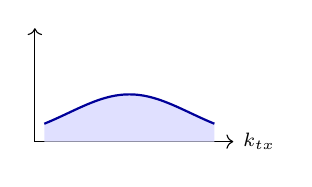
\begin{tikzpicture}[scale=0.6]
				\draw[->] (0,0) -- (4.2,0) node[right, font=\scriptsize] {$k_{tx}$};
				\draw[->] (0,0) -- (0,2.4);
				\fill[blue!12] plot[smooth, domain=0.2:3.8] (\x, {1.0*exp(-0.3*(\x-2)^2)}) -- (3.8,0) -- (0.2,0) -- cycle;
				\draw[thick, blue!60!black] plot[smooth, domain=0.2:3.8] (\x, {1.0*exp(-0.3*(\x-2)^2)});
			\end{tikzpicture}\\
			{\scriptsize\itshape broad --- many values plausible}
		\end{column}
		\begin{column}{0.32\textwidth}
			\centering
			\textbf{Data} $p(\textrm{data} \mid \theta)$\\
			{\scriptsize what the experiment says}
			\medskip\\
			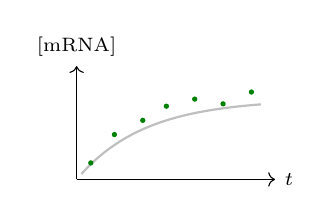
\begin{tikzpicture}[scale=0.6]
				\draw[->] (0,0) -- (4.2,0) node[right, font=\scriptsize] {$t$};
				\draw[->] (0,0) -- (0,2.4) node[above, font=\scriptsize] {[mRNA]};
				\draw[thick, gray!50] plot[smooth, domain=0.1:3.9] (\x, {1.7*(1-exp(-0.7*\x))});
				\foreach \x/\y in {0.3/0.35, 0.8/0.95, 1.4/1.25, 1.9/1.55, 2.5/1.7, 3.1/1.6, 3.7/1.85} {
					\fill[green!50!black] (\x,\y) circle (1.6pt);
				}
			\end{tikzpicture}\\
			{\scriptsize\itshape noisy observations + model}
		\end{column}
		\begin{column}{0.32\textwidth}
			\centering
			\textbf{Posterior} $p(\theta \mid \textrm{data})$\\
			{\scriptsize what to believe after data}
			\medskip\\
			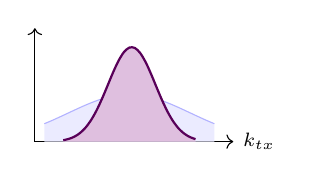
\begin{tikzpicture}[scale=0.6]
				\draw[->] (0,0) -- (4.2,0) node[right, font=\scriptsize] {$k_{tx}$};
				\draw[->] (0,0) -- (0,2.4);
				\fill[blue!8] plot[smooth, domain=0.2:3.8] (\x, {1.0*exp(-0.3*(\x-2)^2)}) -- (3.8,0) -- (0.2,0) -- cycle;
				\draw[thin, blue!30] plot[smooth, domain=0.2:3.8] (\x, {1.0*exp(-0.3*(\x-2)^2)});
				\fill[violet!25] plot[smooth, domain=0.6:3.4] (\x, {2.0*exp(-2.0*(\x-2.05)^2)}) -- (3.4,0) -- (0.6,0) -- cycle;
				\draw[thick, violet!70!black] plot[smooth, domain=0.6:3.4] (\x, {2.0*exp(-2.0*(\x-2.05)^2)});
			\end{tikzpicture}\\
			{\scriptsize\itshape tight --- data has constrained it}
		\end{column}
	\end{columns}
	
	\vfill
	\centering
	$\underbrace{p(\theta \mid \textrm{data})}_{\textrm{posterior}} \;\propto\; \underbrace{p(\textrm{data} \mid \theta)}_{\textrm{likelihood}} \;\cdot\; \underbrace{p(\theta)}_{\textrm{prior}}$
	
	\medskip
	{\small The posterior is the output. Predictions with credible intervals, identifiability, model comparison --- all follow.}
\end{frame}

% ----------------------------------------------------------------
\begin{frame}[noframenumbering]{What Inference Enables}

	Inference lets you ask scientific questions that forward simulation cannot pose.

	\bigskip
	\small
	\begin{columns}[T]
		\begin{column}{0.58\textwidth}
			\begin{enumerate}\itemsep8pt
				\item \textbf{Are my predictions trustworthy?}\\
				{\small Propagate parameter uncertainty to get credible intervals on outputs. Robust predictions vs. fragile ones.}

				\item \textbf{What biology can I learn?}\\
				{\small Bayesian model selection. Posteriors on shared parameters reveal how subsystems interact.}

				\item \textbf{What can I learn about my model?}\\
				{\small Which parameters are identifiable? Does the formalism matter (ODE vs SSA)? Where does the model fail to reproduce data? What experiment should you run next?}
			\end{enumerate}
		\end{column}
		\begin{column}{0.38\textwidth}
			\centering
			% 1. Predictions with uncertainty
			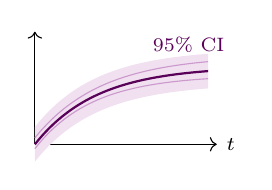
\begin{tikzpicture}[scale=0.55]
				\draw[->] (0,0) -- (4.2,0) node[right, font=\scriptsize] {$t$};
				\draw[->] (0,0) -- (0,2.6);
				\fill[violet!12] plot[smooth, domain=0:4] (\x, {1.8*(1-exp(-0.7*\x)) + 0.4})
					-- plot[smooth, domain=4:0] (\x, {1.8*(1-exp(-0.7*\x)) - 0.4}) -- cycle;
				\draw[thin, violet!40] plot[smooth, domain=0:4] (\x, {1.9*(1-exp(-0.65*\x)) + 0.15});
				\draw[thin, violet!40] plot[smooth, domain=0:4] (\x, {1.7*(1-exp(-0.75*\x)) - 0.1});
				\draw[thick, colPostLine] plot[smooth, domain=0:4] (\x, {1.8*(1-exp(-0.7*\x))});
				\node[font=\scriptsize, colPostLine, anchor=west] at (2.5,2.3) {95\% CI};
			\end{tikzpicture}

			\vspace{6pt}

			% 2. Mechanistic inference: model selection
			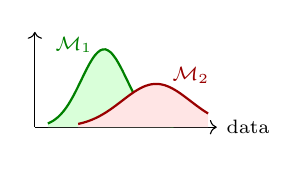
\begin{tikzpicture}[scale=0.55]
				\draw[->] (0,0) -- (4.2,0) node[right, font=\scriptsize] {data};
				\draw[->] (0,0) -- (0,2.2);
				\fill[green!15] plot[smooth, domain=0.3:3.2] (\x, {1.8*exp(-1.8*(\x-1.6)^2)}) -- (3.2,0) -- (0.3,0) -- cycle;
				\draw[thick, green!50!black] plot[smooth, domain=0.3:3.2] (\x, {1.8*exp(-1.8*(\x-1.6)^2)});
				\fill[red!10] plot[smooth, domain=1.0:4.0] (\x, {1.0*exp(-0.8*(\x-2.8)^2)}) -- (4.0,0) -- (1.0,0) -- cycle;
				\draw[thick, red!60!black] plot[smooth, domain=1.0:4.0] (\x, {1.0*exp(-0.8*(\x-2.8)^2)});
				\node[font=\scriptsize, green!50!black] at (0.9,1.9) {$\mathcal{M}_1$};
				\node[font=\scriptsize, red!60!black] at (3.6,1.2) {$\mathcal{M}_2$};
			\end{tikzpicture}

			\vspace{6pt}

			% 3. Learn about model: identifiability (posterior vs prior)
			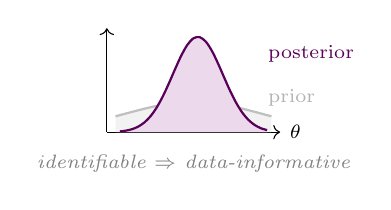
\begin{tikzpicture}[scale=0.55]
				\draw[->] (0,0) -- (4,0) node[right, font=\scriptsize] {$\theta$};
				\draw[->] (0,0) -- (0,2.4);
				% Broad prior
				\fill[gray!10] plot[smooth, domain=0.2:3.8] (\x, {0.7*exp(-0.2*(\x-2)^2)}) -- (3.8,0) -- (0.2,0) -- cycle;
				\draw[thick, gray!50] plot[smooth, domain=0.2:3.8] (\x, {0.7*exp(-0.2*(\x-2)^2)});
				% Tight posterior
				\fill[colPost] plot[smooth, domain=0.3:3.7] (\x, {2.2*exp(-1.5*(\x-2.1)^2)}) -- (3.7,0) -- (0.3,0) -- cycle;
				\draw[thick, colPostLine] plot[smooth, domain=0.3:3.7] (\x, {2.2*exp(-1.5*(\x-2.1)^2)});
				\node[font=\scriptsize, gray!60, anchor=west] at (3.5,0.8) {prior};
				\node[font=\scriptsize, colPostLine, anchor=west] at (3.5,1.8) {posterior};
				\node[font=\scriptsize\itshape, gray, anchor=north] at (2,-0.3) {identifiable $\Rightarrow$ data-informative};
			\end{tikzpicture}
		\end{column}
	\end{columns}
\end{frame}


% ================================================================
% Problem deep-dives: why current WCMs cannot deliver inference
% ================================================================

% ----------------------------------------------------------------
\begin{frame}
		{\scriptsize\itshape MC4D: 50 replicate sims, \emph{same} $\boldsymbol{\theta}$ \textcolor{blue!70!black}{(aleatoric only)}}
	
	
	
	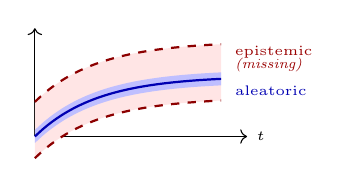
\begin{tikzpicture}[scale=0.55]
		\draw[->] (0,0) -- (4.9,0) node[right, font=\tiny] {$t$};
		\draw[->] (0,0) -- (0,2.5);
		% Wide epistemic band (imagined, missing in MC4D)
		\fill[red!10] plot[smooth, domain=0:4.3] (\x, {1.4*(1-exp(-0.7*\x)) + 0.8}) --
		plot[smooth, domain=4.3:0] (\x, {1.4*(1-exp(-0.7*\x)) - 0.5}) -- cycle;
		\draw[thick, dashed, red!55!black] plot[smooth, domain=0:4.3] (\x, {1.4*(1-exp(-0.7*\x)) + 0.8});
		\draw[thick, dashed, red!55!black] plot[smooth, domain=0:4.3] (\x, {1.4*(1-exp(-0.7*\x)) - 0.5});
		% Narrow aleatoric band (real)
		\fill[blue!25] plot[smooth, domain=0:4.3] (\x, {1.4*(1-exp(-0.7*\x)) + 0.15}) --
		plot[smooth, domain=4.3:0] (\x, {1.4*(1-exp(-0.7*\x)) - 0.15}) -- cycle;
		% Mean trajectory
		\draw[thick, blue!70!black] plot[smooth, domain=0:4.3] (\x, {1.4*(1-exp(-0.7*\x))});
		% Labels
		\node[font=\tiny, blue!70!black, anchor=west] at (4.4, 1.05) {aleatoric};
		\node[font=\tiny, red!60!black, anchor=west] at (4.4, 1.95) {epistemic};
		\node[font=\tiny\itshape, red!60!black, anchor=west] at (4.4, 1.65) {(missing)};
	\end{tikzpicture}\\[1pt]
	{\scriptsize\itshape Schematic: \textcolor{red!60!black}{\textbf{parameter uncertainty}} would widen the band}
\end{frame}

% ----------------------------------------------------------------
\begin{frame}[noframenumbering]{Implications of Root 1: No Probabilistic Information Flow (1/2)}
	\scriptsize
	\textit{Standard WCMs have no priors, no likelihood, no posterior --- a deterministic channel from point parameters to point predictions.}

	\smallskip
	\textbf{Forward UQ (priors $\to$ predictions)}
	\begin{itemize}\itemsep0pt\parskip0pt
		\item No credible intervals on observables (doubling time, flux, copy numbers)
		\item Cannot distinguish robust predictions from fragile ones
		\item Cannot quantify prediction risk for downstream use (synbio design, drug targets)
		\item Cannot make calibrated probabilistic claims about cell behaviour
	\end{itemize}

	\smallskip
	\textbf{Inverse inference (data $\to$ parameters)}
	\begin{itemize}\itemsep0pt\parskip0pt
		\item No formal parameter calibration from data --- only ad hoc transfer from related organisms / literature
		\item No joint posteriors $\to$ cannot see how parameters covary
		\item Cannot detect parameter ``bleed-through'' between modules via shared parameters
		\item No principled propagation of experimental uncertainty into the model
		\item No mechanism for Bayesian updating as new data arrives
	\end{itemize}

	\smallskip
	\textbf{Identifiability and structural diagnostics}
	\begin{itemize}\itemsep0pt\parskip0pt
		\item Cannot tell which parameters the data actually constrains
		\item Cannot detect sloppy directions in parameter space (Sethna-style sloppy models)
		\item Cannot detect practical vs.\ structural non-identifiability
		\item Cannot diagnose when nominally distinct parameters are degenerate
	\end{itemize}
\end{frame}

% ----------------------------------------------------------------
\begin{frame}[noframenumbering]{Implications of Root 1: No Probabilistic Information Flow (2/2)}
	\scriptsize
	\textbf{Model criticism and selection}
	\begin{itemize}\itemsep0pt\parskip0pt
		\item No marginal likelihood $\to$ no Bayes factors, no principled model comparison
		\item Cannot compare formalisms (ODE vs SSA vs SDE) on the same data
		\item Cannot run posterior predictive checks to detect misspecification
		\item Cannot detect when literature parameter values are inconsistent with observed data
		\item Cannot test competing mechanistic hypotheses against each other
	\end{itemize}

	\smallskip
	\textbf{Experimental design}
	\begin{itemize}\itemsep0pt\parskip0pt
		\item No Bayesian optimal experimental design (requires expected information gain over posteriors)
		\item Cannot prioritize which parameters to measure next
		\item Cannot quantify the expected value of a new experiment before running it
	\end{itemize}

	\smallskip
	\textbf{Biology discovery}
	\begin{itemize}\itemsep0pt\parskip0pt
		\item Cannot ask ``is mechanism $X$ consistent with the data?'' probabilistically
		\item Cannot quantify evidence for/against alternative mechanisms
		\item Cannot identify gaps in the model where data demands a mechanism not yet included
	\end{itemize}

	\smallskip
	\textbf{Communication and reproducibility}
	\begin{itemize}\itemsep0pt\parskip0pt
		\item Published predictions cannot carry honest uncertainty
		\item Cannot reproduce the \emph{confidence} of a result, only point estimates
	\end{itemize}
\end{frame}

% ----------------------------------------------------------------
\begin{frame}[noframenumbering]{Implications of Root 2: No Unified Execution Substrate (1/2)}
	\footnotesize
	\textit{Standard WCMs span languages, processes, and runtimes --- no single environment for the whole model.}

	\smallskip
	\textbf{Performance / HPC}
	\begin{itemize}\itemsep0pt\parskip0pt
		\item IO and serialization penalties at every module boundary
		\item Subprocess spawn-up cost (LAMMPS, LSODA, Python glue)
		\item Memory copies between runtimes --- no pass-by-reference
		\item Cannot run as a single GPU kernel pipeline
		\item Cannot profile or optimize the whole model as one program
		\item Inter-language data marshalling becomes a bottleneck at scale
	\end{itemize}

	\smallskip
	\textbf{Differentiability and inference efficiency}
	\begin{itemize}\itemsep0pt\parskip0pt
		\item No gradient flow across language boundaries $\to$ no end-to-end AD
		\item Without AD, restricted to gradient-free inference (orders of magnitude more expensive)
		\item Cannot use HMC/NUTS, variational inference, or gradient-based optimization
		\item Cannot do gradient-based sensitivity analysis
		\item Cannot do gradient-based experimental design
	\end{itemize}
\end{frame}

% ----------------------------------------------------------------
\begin{frame}[noframenumbering]{Implications of Root 2: No Unified Execution Substrate (2/2)}
	\scriptsize
	\textbf{Composability and substitution}
	\begin{itemize}\itemsep0pt\parskip0pt
		\item Cannot drop in an ML surrogate for a slow module without cross-language wrapping
		\item Cannot use mixed precision (reduced precision in one module, full in another)
		\item Cannot share a type system across modules (typed states, units, validation)
		\item Cannot reuse infrastructure (logging, checkpointing, error handling) uniformly
		\item Cannot easily try alternative formalisms (swap ODE$\to$SSA) without reimplementation
	\end{itemize}

	\smallskip
	\textbf{Hybrid inference orchestration}
	\begin{itemize}\itemsep0pt\parskip0pt
		\item Cannot mix differentiable and simulation-based inference within one model
		\item No shared substrate for a boundary protocol between blocks
		\item Each inference backend lives in its own ecosystem, not composable
	\end{itemize}

	\smallskip
	\textbf{Software engineering and extensibility}
	\begin{itemize}\itemsep0pt\parskip0pt
		\item Build/install complexity (multiple toolchains, multiple dependency managers)
		\item Debugging and stack traces don't cross language boundaries
		\item Testing infrastructure fragmented across languages
		\item Reproducibility harder (multiple env specs, versions, OS-level dependencies)
		\item New contributors must learn the polyglot stack to add anything
	\end{itemize}

	\smallskip
	\textbf{Scientific prototyping}
	\begin{itemize}\itemsep0pt\parskip0pt
		\item Adding a module commits you to its language's ecosystem
		\item Cannot prototype new ideas cheaply --- every experiment requires cross-language plumbing
		\item Limits who can contribute to model development
	\end{itemize}
\end{frame}

% ----------------------------------------------------------------
\begin{frame}[noframenumbering]{Cross-Cutting: Capabilities That Need Both Roots}
	\footnotesize
	A few headline capabilities require \emph{both} roots to be addressed --- Root 1 makes them definable, Root 2 makes them tractable.

	\medskip
	\begin{itemize}\itemsep6pt
		\item \textbf{Scalable Bayesian inference on a whole-cell model}\\
		{\scriptsize Likelihood (Root 1) $\times$ efficient gradients (Root 2). Neither alone gets you HMC-at-scale.}

		\item \textbf{Joint posteriors over coupled modules}\\
		{\scriptsize Probabilistic semantics (Root 1) $\times$ shared runtime to evaluate them (Root 2). Cross-module dependencies become visible only when both are present.}

		\item \textbf{Gradient-based experimental design at scale}\\
		{\scriptsize Posterior (Root 1) $\times$ AD through the simulator (Root 2). Required for expected information gain over realistic models.}

		\item \textbf{Hybrid inference across heterogeneous blocks}\\
		{\scriptsize Probabilistic boundary protocol (Root 1) $\times$ shared substrate to pass distributions across it (Root 2). Differentiable + simulation-based blocks in one model.}
	\end{itemize}

	\medskip
	\centering
	\alert{These are the capabilities that distinguish InferCell from any architecture addressing only one root.}
\end{frame}


% ================================================================
% Inference payoffs: what posteriors give you that point estimates cannot
% ================================================================

% ----------------------------------------------------------------
\begin{frame}[noframenumbering]{Which Predictions Can You Trust?}
		\footnotesize
	\begin{columns}[T]
		\begin{column}{0.55\textwidth}
			Propagate the posterior through the model.\\Some predictions are \textbf{robust}, others are \textbf{fragile}.

			\bigskip
			\begin{itemize}\itemsep8pt
				\item \textbf{Robust prediction:}\\
				{\small Barely changes across the posterior. You can trust this output regardless of parameter uncertainty.}

				\item \textbf{Fragile prediction:}\\
				{\small Swings wildly. Sensitive to parameters the data cannot constrain. This is where you need more data --- or a simpler model.}
			\end{itemize}

			\bigskip
			{\small Forward simulation never tells you which is which. Every prediction looks equally confident.}
		\end{column}
		\begin{column}{0.42\textwidth}
			\centering
			% Robust prediction: tight band
			\textbf{\small Robust}\\[4pt]
			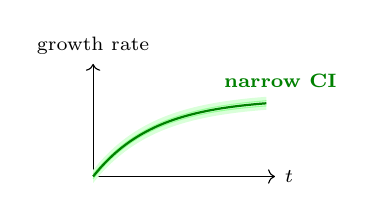
\begin{tikzpicture}[scale=0.55]
				\draw[->] (0,0) -- (4.2,0) node[right, font=\scriptsize] {$t$};
				\draw[->] (0,0) -- (0,2.6) node[above, font=\scriptsize] {growth rate};
				\fill[green!15] plot[smooth, domain=0:4] (\x, {1.8*(1-exp(-0.7*\x)) + 0.15})
					-- plot[smooth, domain=4:0] (\x, {1.8*(1-exp(-0.7*\x)) - 0.15}) -- cycle;
				\draw[thin, green!40] plot[smooth, domain=0:4] (\x, {1.82*(1-exp(-0.68*\x)) + 0.05});
				\draw[thin, green!40] plot[smooth, domain=0:4] (\x, {1.78*(1-exp(-0.72*\x)) - 0.05});
				\draw[thick, green!50!black] plot[smooth, domain=0:4] (\x, {1.8*(1-exp(-0.7*\x))});
				\node[font=\scriptsize\bfseries, green!50!black, anchor=west] at (2.8,2.2) {narrow CI};
			\end{tikzpicture}

			\vspace{8pt}

			% Fragile prediction: wide band
			\textbf{\small Fragile}\\[4pt]
			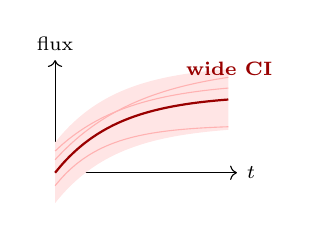
\begin{tikzpicture}[scale=0.55]
				\draw[->] (0,0) -- (4.2,0) node[right, font=\scriptsize] {$t$};
				\draw[->] (0,0) -- (0,2.6) node[above, font=\scriptsize] {flux};
				\fill[red!10] plot[smooth, domain=0:4] (\x, {1.8*(1-exp(-0.7*\x)) + 0.7})
					-- plot[smooth, domain=4:0] (\x, {1.8*(1-exp(-0.7*\x)) - 0.7}) -- cycle;
				\draw[thin, red!30] plot[smooth, domain=0:4] (\x, {2.2*(1-exp(-0.5*\x)) + 0.3});
				\draw[thin, red!30] plot[smooth, domain=0:4] (\x, {1.4*(1-exp(-0.9*\x)) - 0.3});
				\draw[thin, red!30] plot[smooth, domain=0:4] (\x, {1.6*(1-exp(-0.6*\x)) + 0.5});
				\draw[thick, red!60!black] plot[smooth, domain=0:4] (\x, {1.8*(1-exp(-0.7*\x))});
				\node[font=\scriptsize\bfseries, red!60!black, anchor=west] at (2.8,2.4) {wide CI};
			\end{tikzpicture}
		\end{column}
	\end{columns}
\end{frame}

% ----------------------------------------------------------------
\begin{frame}[noframenumbering]{What Your Model Actually Depends On}
	\footnotesize
	\begin{columns}[T]
		\begin{column}{0.55\textwidth}
			With point estimates, every parameter looks equally important.

			\bigskip
			With posteriors, you learn \textbf{which parameters matter}:

			\begin{itemize}\itemsep6pt
				\item \textbf{Tight posterior} (narrower than prior):\\
				{\small Data constrains this parameter. It matters.}

				\item \textbf{Posterior $\approx$ prior:}\\
				{\small Data says nothing. Redundant, or not observable.}

				\item \textbf{Correlated posteriors:}\\
				{\small Parameters trade off. Neither is identifiable alone, but their combination is constrained.}
			\end{itemize}
		\end{column}
		\begin{column}{0.42\textwidth}
			\centering
			% Tight posterior
			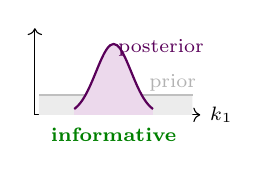
\begin{tikzpicture}[scale=0.5]
				\draw[->] (0,0) -- (4.2,0) node[right, font=\scriptsize] {$k_1$};
				\draw[->] (0,0) -- (0,2.2);
				\fill[gray!15] plot[smooth, domain=0.1:4] (\x, {0.5}) -- (4,0) -- (0.1,0) -- cycle;
				\draw[thick, gray!50] plot[smooth, domain=0.1:4] (\x, {0.5});
				\fill[colPost] plot[smooth, domain=1.0:3.0] (\x, {1.8*exp(-2.5*(\x-2)^2)}) -- (3.0,0) -- (1.0,0) -- cycle;
				\draw[thick, colPostLine] plot[smooth, domain=1.0:3.0] (\x, {1.8*exp(-2.5*(\x-2)^2)});
				\node[font=\scriptsize, gray!60] at (3.5,0.8) {prior};
				\node[font=\scriptsize, colPostLine] at (3.2,1.7) {posterior};
				\node[font=\scriptsize\bfseries, green!50!black] at (2,-0.5) {informative};
			\end{tikzpicture}

			\vspace{6pt}

			% Posterior = prior
			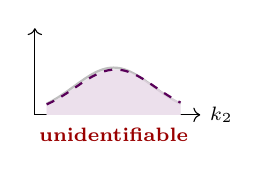
\begin{tikzpicture}[scale=0.5]
				\draw[->] (0,0) -- (4.2,0) node[right, font=\scriptsize] {$k_2$};
				\draw[->] (0,0) -- (0,2.2);
				\fill[gray!15] plot[smooth, domain=0.3:3.7] (\x, {1.2*exp(-0.5*(\x-2)^2)}) -- (3.7,0) -- (0.3,0) -- cycle;
				\draw[thick, gray!50] plot[smooth, domain=0.3:3.7] (\x, {1.2*exp(-0.5*(\x-2)^2)});
				\fill[violet!15, opacity=0.6] plot[smooth, domain=0.3:3.7] (\x, {1.15*exp(-0.48*(\x-2.05)^2)}) -- (3.7,0) -- (0.3,0) -- cycle;
				\draw[thick, colPostLine, dashed] plot[smooth, domain=0.3:3.7] (\x, {1.15*exp(-0.48*(\x-2.05)^2)});
				\node[font=\scriptsize\bfseries, red!60!black] at (2,-0.5) {unidentifiable};
			\end{tikzpicture}

			\vspace{6pt}

			% Correlated posteriors
			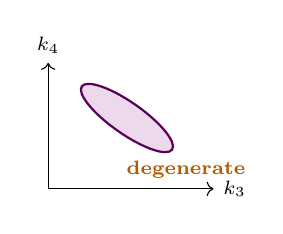
\begin{tikzpicture}[scale=0.5]
				\draw[->] (0,0) -- (4.2,0) node[right, font=\scriptsize] {$k_3$};
				\draw[->] (0,0) -- (0,3.2) node[above, font=\scriptsize] {$k_4$};
				\fill[violet!15, rotate around={-35:(2,1.8)}] (2,1.8) ellipse (1.4 and 0.4);
				\draw[thick, colPostLine, rotate around={-35:(2,1.8)}] (2,1.8) ellipse (1.4 and 0.4);
				\node[font=\scriptsize\bfseries, orange!70!black] at (3.5,0.5) {degenerate};
			\end{tikzpicture}
		\end{column}
	\end{columns}

	\vfill
	\centering
	{\small These are scientific insights --- they tell you what to measure next.\\Forward simulation never reveals them.}
\end{frame}


% ================================================================
% Architecture deep-dives: how the interface, modes, priors, and boundary fit together
% ================================================================

% ----------------------------------------------------------------
\begin{frame}[noframenumbering]{The Interface Is the Architecture}
	\begin{columns}[T]
		\begin{column}{0.55\textwidth}
			The module internals are swappable by design.\\
			What makes inference compose is the \textbf{boundary contract}:

			\medskip
			\begin{itemize}\itemsep6pt
				\item \textbf{States} --- typed variables in, typed variables out
				\item \textbf{Parameters} --- each carries a prior distribution
				\item \textbf{Formalism} --- \texttt{:ode}, \texttt{:sde}, \texttt{:jump}
				\item \textbf{Inference mode} --- \texttt{:differentiable} or \texttt{:simulation}
			\end{itemize}

		\end{column}
		\begin{column}{0.42\textwidth}
			\centering
			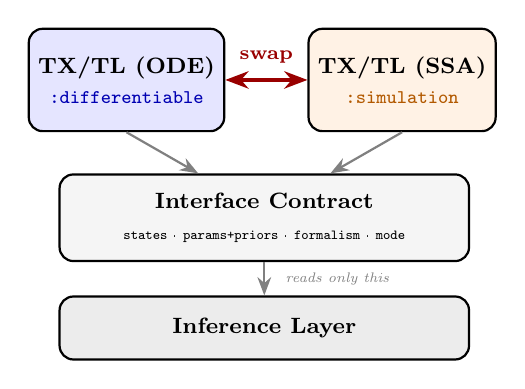
\begin{tikzpicture}[
				scale=0.7,
				>=Stealth
			]
				\node[draw, thick, rounded corners=5pt, fill=blue!10,
					minimum height=1.3cm, minimum width=2.3cm, align=center]
					(v1) at (-2.5, 4) {%
						\footnotesize\textbf{TX/TL (ODE)}\\[-1pt]
						{\scriptsize\color{blue!70!black}\texttt{:differentiable}}};

				\node[draw, thick, rounded corners=5pt, fill=orange!10,
					minimum height=1.3cm, minimum width=2.3cm, align=center]
					(v2) at (2.5, 4) {%
						\footnotesize\textbf{TX/TL (SSA)}\\[-1pt]
						{\scriptsize\color{orange!70!black}\texttt{:simulation}}};

				\draw[<->, very thick, red!60!black] (v1.east) -- (v2.west)
					node[midway, above=2pt, font=\scriptsize\bfseries, text=red!60!black] {swap};

				\node[draw, thick, rounded corners=5pt, fill=gray!8,
					minimum height=1.1cm, minimum width=5.2cm, align=center]
					(iface) at (0, 1.5) {%
						\footnotesize\textbf{Interface Contract}\\[-1pt]
						{\tiny\texttt{states\;\textperiodcentered\;params+priors\;\textperiodcentered\;formalism\;\textperiodcentered\;mode}}};

				\draw[->, thick, gray] (v1.south) -- ([xshift=-1.2cm]iface.north);
				\draw[->, thick, gray] (v2.south) -- ([xshift=1.2cm]iface.north);

				\node[draw, thick, rounded corners=5pt, fill=colNeutral,
					minimum height=0.8cm, minimum width=5.2cm,
					font=\footnotesize\bfseries]
					(inf) at (0, -0.5) {Inference Layer};

				\draw[->, thick, gray] (iface.south) -- (inf.north)
					node[midway, right=4pt, font=\tiny\itshape, text=gray] {reads only this};
			\end{tikzpicture}
		\end{column}
	\end{columns}
\vspace{1mm}
The inference layer sees \emph{only} the interface. It never looks inside the module.


	\alert{Design test: can you swap the internals without changing the inference call?}
\end{frame}

% ----------------------------------------------------------------
\begin{frame}[noframenumbering,fragile]{Modules Declare Their Inference Mode}
	Each module is defined by a \textbf{typed interface} that declares its dynamics \emph{and} how inference should work:

	\bigskip
	\begin{columns}[T]
		\begin{column}{0.52\textwidth}
			\begin{lstlisting}[style=julia]
abstract type AbstractSubModel end

states(m)          # state variables
parameters(m)      # with priors
dynamics(u, p, t, m)  # rate equations
formalism(m)       # :ode, :sde, :jump
inference_mode(m)  # :differentiable,
                   # :simulation, :auto
			\end{lstlisting}
		\end{column}
		\begin{column}{0.45\textwidth}
			\begin{itemize}\itemsep6pt
				\item The framework reads these declarations and \textbf{automatically partitions} modules into the right inference backend
				\item Adding a module extends the inference problem \textbf{without code changes} to the inference layer
				\item Swap an ODE model for an SSA model --- the backend switches automatically
			\end{itemize}
		\end{column}
	\end{columns}

	\vfill
	\centering
	\alert{Modularity at the inference level, not just the simulation level.}
\end{frame}

% ----------------------------------------------------------------
\begin{frame}[noframenumbering,fragile]{Parameters Carry Priors}
	Every parameter declares its value, prior distribution, and whether it is free or fixed:

	\bigskip
	\begin{columns}[T]
		\begin{column}{0.48\textwidth}
			\begin{lstlisting}[style=julia]
struct InferParameter
  value::Float64
  prior::Distribution
  fixed::Bool
  name::Symbol
  role::Symbol  # :rate, :initial,
                # :observation
end
			\end{lstlisting}
		\end{column}
		\begin{column}{0.48\textwidth}
			\begin{itemize}\itemsep6pt
				\item \textbf{Fixed:} point estimate from literature
				\item \textbf{Constrained:} informative prior from experiment
				\item \textbf{Free:} to be inferred from data
				\item The inference layer reads these declarations and builds the Bayesian model automatically
				\item Sensitivity analysis is a flag toggle, not a code change
			\end{itemize}
		\end{column}
	\end{columns}
\end{frame}

% ----------------------------------------------------------------
\begin{frame}[noframenumbering]{Boundary Protocol: Three Levels}
	\begin{enumerate}\itemsep8pt
		\item \textbf{Level 1 --- Sequential conditioning (v1 target)}\\
		Infer differentiable block $\to$ posterior samples $\to$ condition simulation block on those samples.\\
		{\small One-directional. Produces a cut posterior. Valid under conditional independence.}

		\item \textbf{Level 2 --- Gibbs-like alternation (v1 demonstration)}\\
		Alternate: fix stochastic module state $\to$ NUTS on differentiable params; fix differentiable params $\to$ SBI on stochastic params.\\
		{\small Bidirectional. Pseudo-marginal Gibbs sampler. Convergence depends on ABC tolerance.}

		\item \textbf{Level 3 --- Particle MCMC (future work)}\\
		Stochastic modules contribute unbiased likelihood estimates via particle filters into a joint MCMC sampler.\\
		{\small Asymptotically exact. Computationally expensive.}
	\end{enumerate}
\end{frame}

% ----------------------------------------------------------------
\begin{frame}[noframenumbering,fragile]{End-to-End Workflow}
	\begin{lstlisting}[style=julia]
using InferCell

# 1. Define sub-model
txl = TranscriptionTranslation()

# 2. Build problem (orchestrator composes modules)
prob = build_problem([txl]; tspan=(0.0, 100.0))

# 3. Generate synthetic data
true_sol = solve(prob, Tsit5())
data = observe(true_sol, 0.0:5.0:100.0; sigma=0.1)

# 4. Infer parameters (NUTS via Turing.jl)
chain = infer(txl, data)

# 5. Posterior predictive check
ppc = posterior_predictive(txl, chain)
	\end{lstlisting}

	\medskip
	{\small Same \texttt{infer()} call works for a single module or a composed multi-module model.}
\end{frame}


% ================================================================
% Concrete module specifications: equations and priors used in the toy WCM
% ================================================================

% ----------------------------------------------------------------
\begin{frame}[noframenumbering]{TX/TL Module: Equations \& Priors}
	\small
	Two-state ODE per gene; four rate parameters plus observation noise:
	\begin{align*}
		\frac{d[\text{mRNA}]}{dt} &= k_{tx} - \gamma_{mRNA} \cdot [\text{mRNA}] \\[6pt]
		\frac{d[\text{protein}]}{dt} &= k_{tl} \cdot [\text{mRNA}] - \gamma_{prot} \cdot [\text{protein}]
	\end{align*}

	\medskip
	\begin{tabular}{lll}
		\toprule
		\textbf{Parameter} & \textbf{Description} & \textbf{Prior} \\
		\midrule
		$k_{tx}$ & Transcription rate & $\text{LogNormal}(0,\;1)$ \\
		$k_{tl}$ & Translation rate & $\text{LogNormal}(0,\;1)$ \\
		$\gamma_{mRNA}$ & mRNA degradation rate & $\text{LogNormal}(0,\;1)$ \\
		$\gamma_{prot}$ & Protein degradation rate & $\text{LogNormal}(0,\;1)$ \\
		$\sigma_{obs}$ & Observation noise & $\text{Normal}(0,\;1)$ truncated $\geq 0$ \\
		\bottomrule
	\end{tabular}

	\medskip
	{\scriptsize Initial conditions $\text{mRNA}_0,\;\text{prot}_0$ declared with $\text{Normal}(0,\;1)$ priors, flagged fixed by default (toggleable).\\Multi-gene variant: per-gene rates and ICs; one shared $\sigma_{obs}$.}
\end{frame}

% ----------------------------------------------------------------
\begin{frame}[noframenumbering]{Metabolism Module: Equations \& Priors}
	\footnotesize
	Three-state ODE (ATP, NTP, AA) with enzyme-modulated ATP production. Inputs from TX/TL: mRNA, enzyme-protein $E$.
	\begin{align*}
		\frac{d[\text{ATP}]}{dt} &= k_{atp}\!\left(1 + \tfrac{E}{K_M + E}\right)\!(\text{ATP}_{\max} - \text{ATP}) - e_{tx} k_{tx} - e_{tl} k_{tl}[\text{mRNA}] - k_{ntp}\,\text{ATP} - k_{aa}\,\text{ATP} \\[2pt]
		\frac{d[\text{NTP}]}{dt} &= k_{ntp}\,\text{ATP} - n_{tx} k_{tx} - \gamma_{ntp}\,\text{NTP} \\[2pt]
		\frac{d[\text{AA}]}{dt}  &= k_{aa}\,\text{ATP} - n_{tl} k_{tl}[\text{mRNA}] - \gamma_{aa}\,\text{AA}
	\end{align*}

	\smallskip
	\begin{tabular}{lll}
		\toprule
		\textbf{Free parameter} & \textbf{Description} & \textbf{Prior} \\
		\midrule
		$k_{atp},\; k_{ntp},\; k_{aa}$ & ATP/NTP/AA synthesis rates & $\text{LogNormal}(0,\;1)$ \\
		$k_{tx}^\star,\; k_{tl}^\star$ & Shared with TX/TL (joint NUTS) & $\text{LogNormal}(0,\;1)$ \\
		$\sigma_{obs}$ & Observation noise & $\text{Normal}(0,\;1)$ truncated $\geq 0$ \\
		\bottomrule
	\end{tabular}

	\smallskip
	{\scriptsize ICs ($\text{Normal}(\cdot,\,1)$, fixed by default): $\text{ATP}_0{=}5,\; \text{NTP}_0{=}2,\; \text{AA}_0{=}2$.\\
	Fixed structural constants: $\text{ATP}_{\max}{=}10,\; e_{tx}{=}0.1,\; e_{tl}{=}0.05,\; n_{tx}{=}n_{tl}{=}0.5,\; \gamma_{ntp}{=}\gamma_{aa}{=}0.1,\; K_M{=}5$.\\
	$^\star$ Shared parameters appear in both TX/TL and Metabolism --- joint NUTS infers a single posterior.}
\end{frame}

% ----------------------------------------------------------------
\begin{frame}[noframenumbering]{Bursty SSA Module: Reactions \& Priors}
	\footnotesize
	Telegraph-promoter gene expression as a jump process. States: $(\text{promoter}\in\{0,1\},\; \text{mRNA},\; \text{protein})$.

	\medskip
	\textbf{Reaction network} (6 \texttt{ConstantRateJump}s):
	\begin{align*}
		\text{(1)}\;\, &\emptyset \to \text{promoter ON} & &\text{rate: } k_{on}\,(1 - \text{promoter}) \\
		\text{(2)}\;\, &\text{promoter ON} \to \emptyset & &\text{rate: } k_{off}\cdot\text{promoter} \\
		\text{(3)}\;\, &\emptyset \to \text{mRNA} & &\text{rate: } k_{tx,\text{burst}}\cdot\text{promoter} \\
		\text{(4)}\;\, &\text{mRNA} \to \emptyset & &\text{rate: } \gamma_{mRNA}\cdot\text{mRNA} \\
		\text{(5)}\;\, &\emptyset \to \text{protein} & &\text{rate: } k_{tl}\cdot\text{mRNA} \\
		\text{(6)}\;\, &\text{protein} \to \emptyset & &\text{rate: } \gamma_{prot}\cdot\text{protein}
	\end{align*}

	\medskip
	\begin{tabular}{lll}
		\toprule
		\textbf{Free parameter} & \textbf{Description} & \textbf{Prior} \\
		\midrule
		$k_{on},\; k_{off}$ & Promoter switching rates & $\text{LogNormal}(0,\;1)$ \\
		$k_{tx,\text{burst}}$ & Burst transcription rate & $\text{LogNormal}(0,\;1)$ \\
		$k_{tl}^\star,\; \gamma_{mRNA}^\star,\; \gamma_{prot}^\star$ & Shared with TX/TL (cross-formalism) & $\text{LogNormal}(0,\;1)$ \\
		\bottomrule
	\end{tabular}

	\smallskip
	{\scriptsize ICs ($\text{Normal}(0,\,1)$, fixed by default): $\text{promoter}_0,\;\text{mRNA}_0,\;\text{protein}_0$.\\
	Inference: ABC-SMC on summary statistics --- no explicit likelihood. $^\star$ shared params receive conditioned priors from the DifferentiableBlock posterior via the boundary protocol.}
\end{frame}


% ================================================================
% Status and positioning: where v0.0.1 sits relative to existing work
% ================================================================

% ----------------------------------------------------------------
\begin{frame}[noframenumbering]{v0.0.1: Implementation Status (May 2026)}
	\begin{columns}[T]
		\begin{column}{0.45\textwidth}
			\footnotesize
			\textbf{Modules}
			\begin{itemize}\itemsep1pt\parskip0pt
				\item TX/TL (ODE), multi-gene
				\item Metabolism (ODE), $+$ enzyme feedback
				\item Bursty SSA, telegraph promoter
			\end{itemize}

			\smallskip
			\textbf{Block inference}
			\begin{itemize}\itemsep1pt\parskip0pt
				\item DifferentiableBlock $\to$ joint NUTS
				\item SimulationBlock $\to$ ABC-SMC
			\end{itemize}

			\smallskip
			\textbf{Boundary protocol}
			\begin{itemize}\itemsep1pt\parskip0pt
				\item Level 1 (cut posterior) $\checkmark$
				\item Level 2 (iterative, KL-converged) $\checkmark$
			\end{itemize}

			\smallskip
			\textbf{Robustness}
			\begin{itemize}\itemsep1pt\parskip0pt
				\item Tier B mismatch generator
			\end{itemize}
		\end{column}
		\begin{column}{0.52\textwidth}
			\centering
			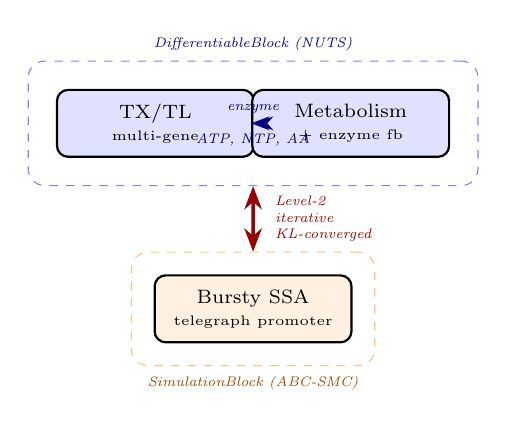
\begin{tikzpicture}[
				scale=0.62,
				mod/.style={draw, thick, rounded corners=4pt, minimum height=0.85cm, minimum width=2.5cm, align=center, font=\scriptsize},
				>=Stealth
			]
				\node[mod, fill=blue!12] (txl) at (0,1) {TX/TL\\\tiny multi-gene};
				\node[mod, fill=blue!12] (met) at (4,1) {Metabolism\\\tiny $+$ enzyme fb};
				\draw[<->, thick, blue!50!black] (txl.east) -- (met.west)
					node[midway, above, font=\tiny\itshape] {enzyme}
					node[midway, below, font=\tiny\itshape] {ATP, NTP, AA};

				\node[mod, fill=orange!12] (ssa) at (2,-2.8) {Bursty SSA\\\tiny telegraph promoter};

				\node[draw, dashed, blue!50, rounded corners=6pt, fit=(txl)(met), inner sep=10pt,
				      label={[font=\tiny\itshape, text=blue!60!black]above:DifferentiableBlock (NUTS)}] (diffblock) {};
				\node[draw, dashed, orange!50, rounded corners=6pt, fit=(ssa), inner sep=8pt,
				      label={[font=\tiny\itshape, text=orange!60!black]below:SimulationBlock (ABC-SMC)}] (simblock) {};

				\draw[<->, very thick, red!60!black] (diffblock.south) -- (simblock.north)
					node[midway, right=4pt, font=\tiny\itshape, align=left]
					{Level-2\\iterative\\KL-converged};
			\end{tikzpicture}
		\end{column}
	\end{columns}

	\vfill
	\centering
	\alert{\itshape Integration test (Slurm, $\sim$32 min): Level-2 narrows shared-param 90\% CIs by $>$50\% vs single-pass.}
\end{frame}



% ================================================================
% Engineering and computational backing: how this is made tractable
% ================================================================

% ----------------------------------------------------------------
\begin{frame}[noframenumbering]{GPU Acceleration and the Julia Advantage}
		\scriptsize
	\begin{columns}[T]
		\begin{column}{0.42\textwidth}
			\textbf{The bottleneck:} every NUTS leapfrog step solves the full ODE system. As models grow, this means $O(10^4)$ ODE solves per chain.

			\bigskip
			\textbf{Julia's single-language stack:}
			\begin{itemize}\itemsep4pt
				\item \textbf{DiffEqGPU.jl}: batch ODE solves on GPU --- same code, one-line backend switch
				\item \textbf{AD composes with GPU kernels}: gradients through GPU-accelerated solvers, no custom CUDA
				\item \textbf{KernelAbstractions.jl}: write once, run on CUDA, ROCm, Metal, or CPU
			\end{itemize}

			\bigskip
			{\small No serialisation between sampler $\leftrightarrow$ solver $\leftrightarrow$ GPU. One compiled representation top to bottom.}
		\end{column}
		\begin{column}{0.55\textwidth}
			\centering
			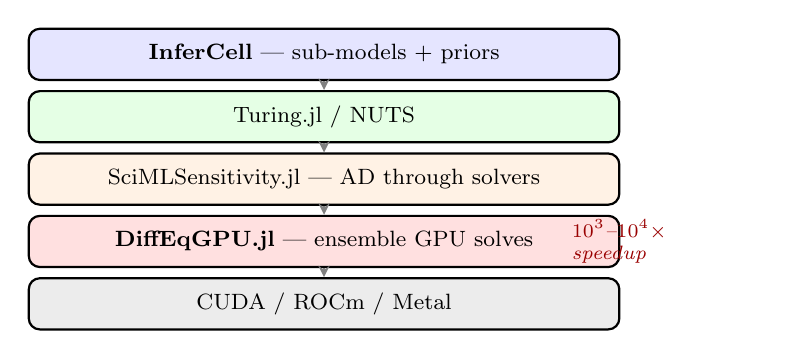
\begin{tikzpicture}[
				scale=0.72,
				layer/.style={draw, thick, rounded corners=4pt, minimum height=0.65cm, minimum width=7.5cm, align=center, font=\footnotesize},
				>=Stealth
			]
				\node[layer, fill=blue!10] (app) at (0,2.6) {\textbf{InferCell} --- sub-models + priors};
				\node[layer, fill=green!10] (inf) at (0,1.5) {Turing.jl / NUTS};
				\node[layer, fill=orange!10] (ad) at (0,0.4) {SciMLSensitivity.jl --- AD through solvers};
				\node[layer, fill=red!12] (gpu) at (0,-0.7) {\textbf{DiffEqGPU.jl} --- ensemble GPU solves};
				\node[layer, fill=gray!15] (hw) at (0,-1.8) {CUDA / ROCm / Metal};
				\draw[pipelinearr, gray] (app) -- (inf);
				\draw[pipelinearr, gray] (inf) -- (ad);
				\draw[pipelinearr, gray] (ad) -- (gpu);
				\draw[pipelinearr, gray] (gpu) -- (hw);
				\node[font=\scriptsize\itshape, text=red!60!black, anchor=west] at (4.2,-0.7) {\parbox{2.5cm}{$10^3$--$10^4\times$\\speedup}};
			\end{tikzpicture}

			\bigskip
			\textbf{What this enables:}
			\begin{itemize}\itemsep3pt
				\item Parallel MCMC chains across GPU cores
				\item Posterior predictive checks batched on GPU
				\item Adjoint sensitivity methods scale to 100+ parameters without linear cost growth
			\end{itemize}
		\end{column}
	\end{columns}
\end{frame}

% ----------------------------------------------------------------
\begin{frame}[noframenumbering]{Why Julia (and Not JAX)?}
	\small
	\begin{columns}[T]
		\begin{column}{0.48\textwidth}
			\textbf{Julia wins on composability:}
			\scriptsize
			\begin{itemize}\itemsep3pt
				\item DiffEq + Turing + SciMLSensitivity + Catalyst share one type system --- AD flows end-to-end with no language boundaries
				\item Multiple dispatch makes the \texttt{AbstractSubModel} interface natural: \texttt{formalism(m)} dispatches to the right solver
				\item Catalyst.jl gives a CRN DSL with no JAX equivalent --- critical for structural inference
			\end{itemize}

			\textbf{For v1, Julia is OK:}\\
			{\scriptsize The research contribution is the architecture and boundary protocol, not the scale. Julia lets us express the ideas most directly.}
		\end{column}
		\begin{column}{0.48\textwidth}
			\textbf{JAX would be ahead on:}
			\scriptsize
			\begin{itemize}\itemsep3pt
				\item \textbf{SBI tooling.} Python \texttt{sbi} library is more mature (neural density estimators, normalizing flows)
				\item \textbf{GPU at scale.} XLA compilation, \texttt{vmap}/\texttt{pmap} over samples --- smoother path to 100+ parameters
				\item \textbf{Community.} Larger pool of computational biology contributors
				\item \textbf{ML integration.} Neural surrogates, amortized inference live in PyTorch/JAX
			\end{itemize}

			\medskip
			\textbf{The risk to watch:}\\
			{\scriptsize If InferCell needs neural SBI or heavy GPU batching at whole-cell scale, the ecosystem gap could be annoying.}
		\end{column}
	\end{columns}
\end{frame}


% ================================================================
% Structural (CRN) inference: inferring which reactions exist, not just their rates
% ================================================================

% ----------------------------------------------------------------
\begin{frame}[noframenumbering]{Beyond Parameter Uncertainty: Which Reactions Exist?}
	\small
	\begin{columns}[T]
		\begin{column}{0.55\textwidth}
			So far: \textbf{fixed model structure}, infer rate constants.

			\bigskip
			But often the structure itself is uncertain:
			\begin{itemize}\itemsep6pt
				\item Is gene $X$ regulated by protein $Y$?
				\item Does this metabolite inhibit that enzyme?
				\item Which of several proposed pathways is active?
			\end{itemize}

			\bigskip
			Different CRN structures can fit training data equally well but \textbf{diverge catastrophically under novel conditions}
			{\scriptsize (Foo et al.\ 2025, Fig.~2: reconstruction error small, prediction error 10$\times$ larger for wrong structure).}
		\end{column}
		\begin{column}{0.42\textwidth}
			\centering
			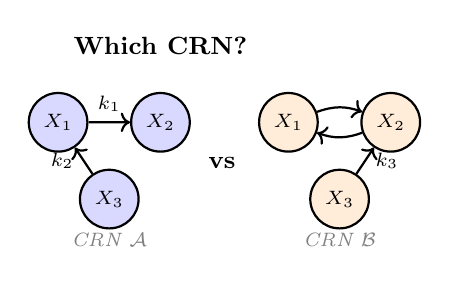
\begin{tikzpicture}[scale=0.65, every node/.style={font=\scriptsize}]
				% Two candidate CRNs
				\node[font=\small\bfseries] at (2,4.5) {Which CRN?};

				% CRN A
				\node[draw, circle, thick, fill=blue!15, minimum size=0.7cm] (a1) at (0,3) {$X_1$};
				\node[draw, circle, thick, fill=blue!15, minimum size=0.7cm] (a2) at (2,3) {$X_2$};
				\node[draw, circle, thick, fill=blue!15, minimum size=0.7cm] (a3) at (1,1.5) {$X_3$};
				\draw[->, thick] (a1) -- (a2) node[midway, above] {$k_1$};
				\draw[->, thick] (a3) -- (a1) node[midway, left] {$k_2$};
				\node[font=\scriptsize\itshape, text=gray] at (1,0.7) {CRN $\mathcal{A}$};

				% vs
				\node[font=\small\bfseries] at (3.2,2.2) {vs};

				% CRN B
				\node[draw, circle, thick, fill=orange!15, minimum size=0.7cm] (b1) at (4.5,3) {$X_1$};
				\node[draw, circle, thick, fill=orange!15, minimum size=0.7cm] (b2) at (6.5,3) {$X_2$};
				\node[draw, circle, thick, fill=orange!15, minimum size=0.7cm] (b3) at (5.5,1.5) {$X_3$};
				\draw[->, thick] (b1) to[bend left=20] (b2);
				\draw[->, thick] (b2) to[bend left=20] (b1);
				\draw[->, thick] (b3) -- (b2) node[midway, right] {$k_3$};
				\node[font=\scriptsize\itshape, text=gray] at (5.5,0.7) {CRN $\mathcal{B}$};
			\end{tikzpicture}

			\medskip
			{\scriptsize Both fit the data.\\Only one predicts correctly\\under new conditions.}
		\end{column}
	\end{columns}

	\vfill
	\centering
	\alert{Structural uncertainty can dominate parameter uncertainty.}
\end{frame}

% ----------------------------------------------------------------
\begin{frame}[noframenumbering]{CRN Inference as a Plug-and-Play Module}
	\footnotesize
	\begin{columns}[T]
		\begin{column}{0.48\textwidth}
			\textbf{Key idea:} include \emph{all} candidate reactions in one module. Let the \textbf{posterior} decide which are present.

			\bigskip
			\begin{itemize}\itemsep6pt
				\item Define a candidate library $\mathcal{R}_{\mathrm{all}}$
				\item Dynamics: $\dot{x}_s = \sum_{r} \nu_{sr}\, k_r \prod_j x_j^{m_{rj}}$
				\item One rate constant $k_r$ per reaction
				\item Horseshoe prior: $k_r \sim \text{HS}(\tau)$\\
				{\small Pushes most $k_r \to 0$}
				\item Posterior over $\mathbf{k}$ \emph{is} the posterior over structures
			\end{itemize}

			\bigskip
			{\small No new inference machinery needed.\\Same \texttt{infer()} call. The prior does the work.}
		\end{column}
		\begin{column}{0.48\textwidth}
			\centering
			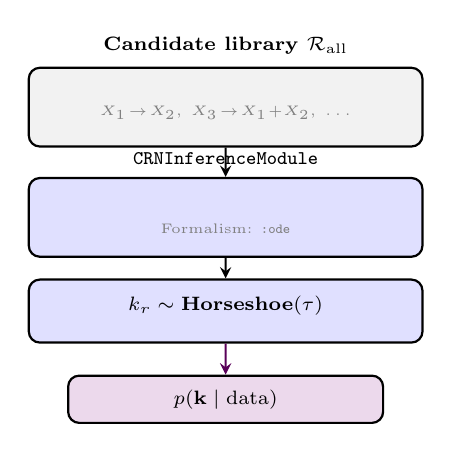
\begin{tikzpicture}[
				scale=0.7,
				mod/.style={draw, thick, rounded corners=4pt, minimum height=0.6cm, align=center, font=\scriptsize},
				>=Stealth
			]
				% Candidate library
				\node[mod, fill=gray!10, minimum width=5cm, minimum height=1cm] (lib) at (2.5,3.5) {};
				\node[above=1pt, font=\scriptsize\bfseries] at (lib.north) {Candidate library $\mathcal{R}_{\mathrm{all}}$};
				\node[font=\tiny, text=gray] at (2.5,3.4) {$X_1 \!\to\! X_2,\; X_3 \!\to\! X_1 \!+\! X_2,\; \ldots$};

				% Module
				\node[mod, fill=blue!12, minimum width=5cm, minimum height=1cm] (crn) at (2.5,1.5) {};
				\node[above=1pt, font=\scriptsize\bfseries] at (crn.north) {\texttt{CRNInferenceModule}};
				\node[font=\tiny, text=gray] at (2.5,1.3) {Formalism: \texttt{:ode}};

				% Parameters
				\node[mod, fill=colODE, minimum width=5cm, minimum height=0.8cm] (params) at (2.5,-0.2) {};
				\node[font=\scriptsize\bfseries] at (2.5,-0.1) {$k_r \sim \text{Horseshoe}(\tau)$};

				% Posterior
				\node[mod, fill=colPost, minimum width=4cm] (post) at (2.5,-1.8) {$p(\mathbf{k} \mid \text{data})$};

				% Arrows
				\draw[pipelinearr] (lib) -- (crn);
				\draw[pipelinearr] (crn) -- (params);
				\draw[pipelinearr, colPostLine] (params) -- (post);
			\end{tikzpicture}
		\end{column}
	\end{columns}
\end{frame}

% ----------------------------------------------------------------
\begin{frame}[noframenumbering]{How the Horseshoe Prior Induces Structure}
		\footnotesize
	\begin{columns}[T]
		\begin{column}{0.50\textwidth}
			The \textbf{horseshoe prior} $k_r \mid \lambda_r \sim \mathcal{N}^+(0, \lambda_r^2 \tau^2)$, $\lambda_r \sim \text{C}^+(0,1)$ has two key properties:

			\begin{enumerate}\itemsep8pt
				\item \textbf{Spike at zero.} Most rate constants are shrunk to effectively zero $\to$ those reactions are ``absent.''
				\item \textbf{Heavy tails.} Reactions that \emph{are} present retain their full magnitude --- minimal bias on the non-zero rates.
			\end{enumerate}

			\bigskip
			The posterior naturally separates into:
			\begin{itemize}\itemsep3pt
				\item $k_r \approx 0$: reaction $r$ absent
				\item $k_r \gg 0$: reaction $r$ present
			\end{itemize}

			\medskip
			{\small\itshape Reaction inclusion probability: $P(r \in \mathcal{R} \mid \text{data}) = P(k_r > \epsilon \mid \text{data})$}
		\end{column}
		\begin{column}{0.46\textwidth}
			\centering
			% Horseshoe prior density sketch
			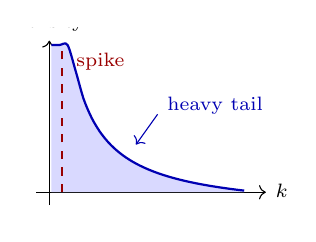
\begin{tikzpicture}[scale=0.55]
				\clip (-0.5,-0.5) rectangle (5.5,3.8);
				\draw[->] (-0.3,0) -- (5,0) node[right, font=\scriptsize] {$k_r$};
				\draw[->] (0,-0.3) -- (0,3.5) node[above, font=\scriptsize] {density};

				% Spike near zero + heavy tail (clipped to axes)
				\fill[blue!15] plot[smooth, domain=0.05:4.5] (\x, {min(3.4, 2.5/(0.15+\x) - 0.5)}) -- (4.5,0) -- (0.05,0) -- cycle;
				\draw[thick, blue!70!black] plot[smooth, domain=0.05:4.5] (\x, {min(3.4, 2.5/(0.15+\x) - 0.5)});

				% Annotations
				\draw[thick, red!60!black, dashed] (0.3,0) -- (0.3,3.4);
				\node[font=\scriptsize, text=red!60!black, anchor=south west] at (0.4,2.6) {spike};
				\node[font=\scriptsize, text=blue!70!black, anchor=west] at (2.5,2) {heavy tail};
				\draw[->, blue!70!black] (2.5,1.8) -- (2,1.1);
			\end{tikzpicture}

			\vspace{4pt}
			% Posterior outcome sketch
			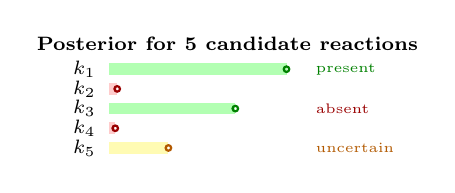
\begin{tikzpicture}[scale=0.5]
				\node[font=\scriptsize\bfseries] at (3,2.8) {Posterior for 5 candidate reactions};
				% k1 - present
				\fill[green!30] (0,2) rectangle (4.5,2.3);
				\draw[thick, green!50!black] (4.5,2.15) circle (2pt);
				\node[font=\scriptsize, anchor=east] at (-0.1,2.15) {$k_1$};
				% k2 - absent
				\fill[red!20] (0,1.5) rectangle (0.2,1.8);
				\draw[thick, red!60!black] (0.2,1.65) circle (2pt);
				\node[font=\scriptsize, anchor=east] at (-0.1,1.65) {$k_2$};
				% k3 - present
				\fill[green!30] (0,1) rectangle (3.2,1.3);
				\draw[thick, green!50!black] (3.2,1.15) circle (2pt);
				\node[font=\scriptsize, anchor=east] at (-0.1,1.15) {$k_3$};
				% k4 - absent
				\fill[red!20] (0,0.5) rectangle (0.15,0.8);
				\draw[thick, red!60!black] (0.15,0.65) circle (2pt);
				\node[font=\scriptsize, anchor=east] at (-0.1,0.65) {$k_4$};
				% k5 - ambiguous
				\fill[yellow!30] (0,0) rectangle (1.5,0.3);
				\draw[thick, orange!70!black] (1.5,0.15) circle (2pt);
				\node[font=\scriptsize, anchor=east] at (-0.1,0.15) {$k_5$};
				% Legend
				\node[font=\tiny, green!50!black, anchor=west] at (5,2.15) {present};
				\node[font=\tiny, red!60!black, anchor=west] at (5,1.15) {absent};
				\node[font=\tiny, orange!70!black, anchor=west] at (5,0.15) {uncertain};
			\end{tikzpicture}
		\end{column}
	\end{columns}
\end{frame}

% ----------------------------------------------------------------
\begin{frame}[noframenumbering]{Relation to Foo et al.\ (2025): Structural Uncertainty in CRNs}
	\scriptsize
	\begin{columns}[T]
		\begin{column}{0.52\textwidth}
			\textbf{Their approach:}
			\begin{enumerate}\itemsep4pt
				\item Sparse optimisation (BFGS) with penalty functions (L1, horseshoe, etc.)
				\item Multiple restarts $\times$ multiple $\lambda$ values
				\item Keep all local optima $\to$ map to CRN structures
				\item BIC approximation for model evidence
				\item Approximate posterior over CRN structures
			\end{enumerate}

			\bigskip
			\textbf{Key results:}
			\begin{itemize}\itemsep3pt
				\item Recovers dynamically equivalent CRNs
				\item Identifies structural ambiguities via posterior correlations
				\item Hierarchical tree of alternative pathways
			\end{itemize}
		\end{column}
		\begin{column}{0.45\textwidth}
			\textbf{Can InferCell do this natively?}
			\begin{itemize}\itemsep6pt
				\item Penalty functions $\to$ \textbf{horseshoe prior}\\
				{\scriptsize Same sparsity, fully Bayesian}
				\item Multi-start optimisation $\to$ \textbf{NUTS sampling}\\
				{\scriptsize Explores multimodal posterior directly}
				\item BIC approximation $\to$ \textbf{exact posterior}\\
				{\scriptsize No need for separate model evidence step}
				\item Separate pruning/recombination pipeline $\to$ \textbf{not needed}\\
				{\scriptsize Posterior samples directly encode structure}
			\end{itemize}

		
		\end{column}
	\end{columns}

	\vfill
	\centering
	{\small Foo, Zanca, Flegg \& Siekmann (2025). \textit{Quantifying structural uncertainty in chemical reaction network inference.} arXiv:2505.15653.}
\end{frame}

% ----------------------------------------------------------------
\begin{frame}[noframenumbering]{Composing Structural Inference with the Inference Graph}
	\begin{columns}[T]
		\begin{column}{0.48\textwidth}
			\small
			Structural inference plugs into the full InferCell architecture:

			\medskip
			\begin{itemize}\itemsep6pt
				\item \textbf{Stage 1:} Discover which reactions are active from data (CRN inference module)
				\item \textbf{Stage 2:} Full Bayesian inference on the discovered structure, composed with other modules
				\item Or run both simultaneously --- horseshoe parameters live alongside standard rate constants in the same NUTS sampler
			\end{itemize}
		\end{column}
		\begin{column}{0.48\textwidth}
			\centering
			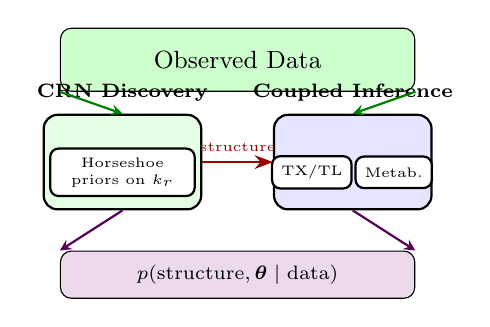
\begin{tikzpicture}[
				scale=0.65,
				block/.style={draw, thick, rounded corners=5pt, minimum height=1.2cm, minimum width=2cm, align=center, font=\scriptsize},
				smallmod/.style={draw, rounded corners=3pt, minimum height=0.4cm, font=\tiny, fill=white, thick},
				>=Stealth
			]
				% Data at top
				\node[pipelinebox=colData, minimum width=4.5cm] (data) at (2.25,5) {Observed Data};

				% CRN Discovery block
				\node[block, fill=green!10] (disc) at (0,3) {};
				\node[above=1pt, font=\scriptsize\bfseries] at (disc.north) {CRN Discovery};
				\node[smallmod] at (0,2.8) {\parbox{1.6cm}{\centering Horseshoe\\priors on $k_r$}};

				% Coupled Inference block
				\node[block, fill=blue!10] (std) at (4.5,3) {};
				\node[above=1pt, font=\scriptsize\bfseries] at (std.north) {Coupled Inference};
				\node[smallmod] (tx) at (3.7,2.8) {TX/TL};
				\node[smallmod] (met) at (5.3,2.8) {Metab.};

				% Data -> blocks
				\draw[pipelinearr, colDataLine] (data.south west) -- (disc.north);
				\draw[pipelinearr, colDataLine] (data.south east) -- (std.north);

				% Arrow between blocks
				\draw[->, thick, red!60!black] (disc.east) -- (std.west)
					node[midway, above, font=\tiny] {structure};

				% Joint posterior at bottom
				\node[pipelinebox=colPost, minimum width=4.5cm, minimum height=0.6cm, font=\scriptsize] (out) at (2.25,0.8) {$p(\text{structure}, \boldsymbol{\theta} \mid \text{data})$};
				\draw[pipelinearr, colPostLine] (disc.south) -- (out.north west);
				\draw[pipelinearr, colPostLine] (std.south) -- (out.north east);
			\end{tikzpicture}
		\end{column}
	\end{columns}
\end{frame}

\backupend

\end{document}
